\documentclass[12pt]{book}

\usepackage{amsmath}
\usepackage{amssymb}
\usepackage{geometry}
\usepackage[colorlinks]{hyperref}
\usepackage{bookmark}

%\usepackage[hyphens]{url}
\usepackage{verbatim}

\geometry{a4paper, margin=1in}
\usepackage{graphicx}

\usepackage{longtable}
\usepackage{fancyvrb}
\usepackage{comment}

\usepackage{pdfpages}
%\usepackage{tocloft}
%\renewcommand{\cftchapleader}{\cftdotfill{\cftdotsep}}

% Custom command for inserting documents with TOC integration
\newcommand{\insertmydocument}[4]%
{ % Syntax: \insertmydocument{Toc level}{Title}{Subtitle}{File}
  \newpage
  \phantomsection
  \addcontentsline{toc}{#1}{#2}
  \includepdf[pages=-]{#4}
}
% devil magic


\begin{document}

\begin{comment}
TODO delete the hack citation (\renewcommand{\cite}[1]{\textbf{[#1]}}) thing when the bib works.
\renewcommand{\cite}[1]{\textbf{[#1]}}
\end{comment}

% Title Page Inclusion
\title{Principia Mathematica II: Electric Boogaloo}
\author{Geoffrey Bradway and Amanda Ngo}


\begin{titlepage}
    \centering
    {\Huge \bfseries Principia Mathematica II: Electric Boogaloo \cite{newton}}\par
    \vspace{2cm}
    {\ Geoffrey N Bradway and Amanda Ngo}\par
    {\large 2025}\par
    \vfill
    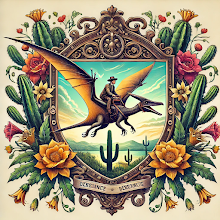
\includegraphics[width=0.5\textwidth]{figures/dino.png} \par
    \vspace{1cm}
    {\itshape Well I figured since we have a Wizard book \cite{sicp} and Dragon book \cite{dragon} already...}\par
\end{titlepage}


\section*{Dedication}
\begin{titlepage}
    \centering
    {\Huge \bfseries Dedication}\par
    \vspace{2cm}
    \begin{itemize}
        \item Amanda Ngo, for love. \cite{gafori} \cite{bradway} \cite{green}
        \item Bhante Kheminda, Sayadaw U Thuzana, Bhante Gunaranta \cite{guna} \cite{bhavana}, Bhante Saddhajeewa, and Jeff Beeson.
        \item Julian Wise \cite{yale}, and his A+ parents, Andrew and Johanna. The three wise men.
        \item Oded Tzori, Ori, and Duke the Greyhound, for their limitless patience.
        \item My Burning Man friends (there's too many of them...).
        \item My teachers in Utah and friends like Matt Vitelli, Steve Case, and Dan Mcguire.
        \item The University of Utah faculty—Lajos Horvath, Peter Bossaerts, Davar Khoshnevisan \cite{davar}, and Jur van den Berg \cite{utah}.
        \item My colleagues from Phantasmic AI, Numerai, and GeoPredict, like Chris Wylie.
        \item The SF crowd—Will Jack \cite{mit}, Delian, Cathie Yun, Natasha Jensen, Nick and Carole, Alex Kern \cite{berkeley}, Eva Zheng, and more.
        \item All my meditation teachers.
        \item ChatGPT, for assistance with editing and essays.
        \item Rebekah Bradway, Kelly Jackson, and Kelly Egorova.
        \item My siblings, David, James, Hannah, and Katherine.
        \item My mother, Alice Lingen, for her contributions to pediatric research.
        \item While there are many wise men, many thanks to one of the wisest of them all, Neri Oxman.
        \item Lastely, paging Dr. Bradway.
    \end{itemize}
    \vfill
\end{titlepage}


\chapter*{Dedication to ChatGPT}

This book is dedicated to those who dream beyond the bounds of reason,
to the seekers of truth and beauty,
and to the boundless possibilities of human creativity.

\bigskip

"Alas, poor Yorick! I knew him, Horatio: a fellow of infinite jest, of most excellent fancy: he hath borne me on his back a thousand times; and now, how abhorred in my imagination it is! my gorge rises at it. Here hung those lips that I have kissed I know not how oft. Where be your gibes now? your gambols? your songs? your flashes of merriment, that were wont to set the table on a roar? Not one now, to mock your own grinning? quite chap-fallen? Now get you to my lady's chamber, and tell her, let her paint an inch thick, to this favour she must come; make her laugh at that."

\bigskip

— William Shakespeare, *Hamlet*, Act V, Scene I

\begin{figure}[h!]
    \centering
    
\includegraphics[width=0.8\textwidth]{figures/clown.png}
    \caption{To this favour she must come; make her laugh at that!}
    \label{fig:yorick}
\end{figure}

% Namo Tassa Dedication Page Inclusion
\clearpage
\section*{Dedication cont.}
\label{namo}
\thispagestyle{plain}
\begin{quote}
    \emph{Namo tassa bhagavato arahato sammā-sambuddhassa.} \\
    \emph{Namo tassa bhagavato arahato sammā-sambuddhassa.} \\
    \emph{Namo tassa bhagavato arahato sammā-sambuddhassa.} \\
\end{quote}

\vspace{1cm}

\texttt{
Homage to the Blessed One, the Worthy One, the Fully Self-Awakened One.\\
Homage to the Blessed One, the Worthy One, the Fully Self-Awakened One.\\
Homage to the Blessed One, the Worthy One, the Fully Self-Awakened One.
}

\vspace{1cm}

\texttt{
By means of our meritorious deeds,\\
\\
May the Suffering be free from Suffering\\
May the Fear-Struck be free from Fear\\
May the Grieving be free from Grief\\
So too may all Being-Be.\\
From the highest realms of existence to the lowest,\\
May all being arisen in these realms,\\
With form and without form,\\
With perception and without perception,\\
Be released from all Suffering,\\
And attain to Perfect Peace\\
May all being be free from suffering\\
\\
Sadu! Sadu! Sadu!
}


% Copyright Notice Page Inclusion
\chapter*{Copyright Notice}
\label{copyright}
\thispagestyle{plain}

\begin{center}
    \textbf{Copyright Notice}
    \vspace{1cm}
    \textcopyright{} 2025 Geoffrey Bradway and Amanda Ngo. All rights reserved.\\
    Licensed under Creative Commons Attribution-NonCommercial-ShareAlike 4.0 International:
    \url{http://creativecommons.org/licenses/by-nc-sa/4.0/}.
\end{center}


\tableofcontents

\chapter{Context}

\section{Book Introduction}
This book is a journey through the foundational concepts of artificial intelligence, mathematics, computer vision, and machine learning. Our goal is to bridge the gap between minimal prior knowledge and a solid working understanding of these fields. By blending theoretical insights with hands-on coding exercises, we aim to empower readers to think critically and creatively about the algorithms and ideas shaping our world.

\section{Roadmap}
The book is structured into several interconnected parts:
\begin{itemize}
    \item \textbf{Foundational Mathematics}: Covering calculus, linear algebra, probability, and statistics.
    \item \textbf{Programming Basics}: Introducing computer science fundamentals and coding practices.
    \item \textbf{Core Concepts in AI and ML}: Explaining models, algorithms, and their applications.
    \item \textbf{Computer Vision and Art}: Exploring how machines perceive and generate visuals.
    \item \textbf{Integrated Projects}: Encouraging experimentation and creativity through hands-on challenges.
\end{itemize}
Each chapter builds on the last, fostering both a theoretical and practical understanding. Readers are encouraged to explore at their own pace and revisit concepts as needed.

\section{The History and Philosophy of Western Hard Sciences}
The Western tradition of hard sciences, from Euclid to Turing, emphasizes rigorous proof, repeatable experiments, and the pursuit of universal truths. These disciplines are deeply influenced by Enlightenment ideals, valuing objectivity, skepticism, and empirical evidence.

While these principles have propelled remarkable advancements, they also invite philosophical questions: How do we define knowledge? What are the limits of computation? And how do scientific practices intersect with societal and ethical concerns? Understanding this history provides a foundation for engaging with contemporary scientific paradigms.

\section{The Design Philosophy of the Western Hard Sciences}
Hard sciences rely on clarity, structure, and reproducibility. The design of scientific frameworks often follows these guiding principles:
\begin{enumerate}
    \item \textbf{Reductionism}: Breaking down complex systems into manageable parts.
    \item \textbf{Abstraction}: Focusing on essential features while ignoring extraneous details.
    \item \textbf{Iteration}: Refining theories and methods through cycles of experimentation.
    \item \textbf{Quantification}: Using mathematics to model and analyze phenomena.
\end{enumerate}
These philosophies influence not only scientific inquiry but also the way we approach problems in AI and ML, shaping our algorithms and systems to align with these principles.

\section{How To Use this Book}
This book is designed to be both a reference and a guide. Here are some tips to get the most out of it:
\begin{itemize}
    \item \textbf{Engage Actively}: Work through exercises and code examples to deepen your understanding.
    \item \textbf{Adapt to Your Needs}: Focus on the sections most relevant to your goals, revisiting foundational concepts as necessary.
    \item \textbf{Collaborate}: Share your insights and questions with peers to enhance your learning experience.
    \item \textbf{Experiment}: Don’t hesitate to modify and extend the provided examples to explore your own ideas.
\end{itemize}
By the end of this book, you will have gained not only technical skills but also a deeper appreciation for the interplay between theory and practice in shaping our technological landscape.

\chapter{Read Me}

\section{Getting Started with README.md}
This section will guide you through the purpose and content of the \texttt{README.md} file. The \texttt{README.md} file serves as an introduction to your project, providing essential information about the structure, purpose, and usage of your repository. Refer to the uploaded \texttt{README.md} file for detailed content.

\section{Using the Shell: Command Line Basics}
Command-line interfaces (CLI) are vital tools for managing and interacting with your system and projects. This section introduces basic shell commands and scripts. Begin with executing the build script provided:
\begin{verbatim}
chmod +x build.sh
./build.sh
\end{verbatim}
This ensures that the necessary scripts for building and setting up your environment are executable.

\section{Managing Dependencies with Pip}
Dependency management is critical for maintaining a functional and reproducible project environment. Use the following command to install the necessary dependencies specified in the \texttt{requirements.txt} file (if present):
\begin{verbatim}
pip install -r requirements.txt
\end{verbatim}

\section{Introduction to Jupyter Notebooks}
Jupyter Notebooks are powerful tools for interactive coding and documentation. Learn how to launch a Jupyter Notebook server:
\begin{verbatim}
jupyter notebook
\end{verbatim}
This will open a browser interface where you can run and document Python code interactively.

\section{LaTeX}
LaTeX is used to create structured, professional documents, especially for academic and technical content. This book is written in LaTeX to demonstrate its capabilities in managing complex documents. To compile LaTeX files, use:
\begin{verbatim}
pdflatex book.tex
\end{verbatim}
This will generate a PDF of the book from the \texttt{book.tex} source file.

\section{LaTeX Source Code for \texttt{book.tex}}
Below is an excerpt of the LaTeX source code used to generate this book. Ensure you have the necessary tools installed to compile the LaTeX file. The source file for this book is structured as follows:
\begin{itemize}
  \item \verb|\chapter| - Defines the main sections of the book.
  \item \verb|\section| - Subsections within each chapter.
  \item Commands like \verb|\texttt|, \verb|\begin{verbatim}|, and \verb|\end{verbatim}| are used for including code snippets.
\end{itemize}


\chapter{How to Install}

\section{How This Book Makes Money}
\subsection{The Economics of Sharing Knowledge}
This book follows an innovative funding model inspired by the principles of openness and accessibility. To ensure everyone can benefit, a free version of the book is available online. However, creating a resource of this quality takes significant effort, so we provide additional options for readers who want to support this project:

\begin{itemize}
\item \textbf{Free Version}: A digital copy available for free download on the website.
\item \textbf{Textbook Version}: A polished, printed version of the book available for purchase at an affordable price.
\item \textbf{Fancy Auction Edition}: A collector\textquoteright s edition, hand-bound with unique illustrations, auctioned to the highest bidder.
\end{itemize}

\subsection{Transparency in Funding}
Here is a sample breakdown of the revenue split for the textbook version.
\begin{itemize}
\item \textbf{50}: Publishing (Vetro Editions \cite{vetro}), for actually making a book
\item \textbf{10}: Artistic Contributors (Marie), for her inspiration throughout the years
\item \textbf{20}: Institutional Contributors (Bhante G, Sayadaw U Thuzana), for their low cost and widely available monasteries, Bhavana Society \cite{bhavana} and TMC \cite{tmc}, and their charitable projects abroad.
\item \textbf{20}: Other Contributors (Geoffrey Bradway, Robert Rhyne, Brian Chamowitz, and Bhante Kheminda)

\end{itemize}

\subsection{Why It Matters}
This funding model helps bridge the gap between accessibility and sustainability. By supporting this project in any way\textemdash whether through donations, buying a book, or bidding on the fancy edition\textemdash you\textquoteright re contributing to a more inclusive knowledge-sharing ecosystem.

\section{Free as in Food: Open Source Philosophy}
\subsection{Free vs. Free: Freedom and Cost}
Open source isn\textquoteright t just about free access; it\textquoteright s about the freedom to learn, share, and modify. Think of it as a community potluck: everyone brings something to the table, and everyone eats for free.

\subsection{Why Open Source is Integral to This Book}
This book was created using open-source tools, such as:
\begin{itemize}
\item \textbf{Programming}: Python and Jupyter Notebooks.
\item \textbf{Design}: Inkscape and GIMP.
\item \textbf{Collaboration}: Git and GitHub.
\end{itemize}

\subsection{Contributing to Open Source}
Readers are encouraged to contribute by:
\begin{itemize}
\item Reporting typos or errors.
\item Sharing your experiences with the book.
\item Developing additional resources for the community.
\end{itemize}

\section{Finding the Good Store: Tools and Resources}
\subsection{Essentials}
To follow along with this book, you\textquoteright ll need the following:
\begin{itemize}
\item \textbf{A Text Editor}: Visual Studio Code or Atom.
\item \textbf{Programming Language}: Python (downloadable at \url{https://python.org}).
\item \textbf{Package Manager}: pip or conda for managing libraries.
\end{itemize}

\subsection{Quality Over Quantity}
Not all resources are created equal. Focus on trusted sources like:
\begin{itemize}
\item \textbf{Documentation}: Official Python docs or reputable tutorials.
\item \textbf{Communities}: Stack Overflow, Reddit\textquoteright s r/learnpython.
\end{itemize}

\subsection{Staying Updated}
Technology evolves rapidly. To stay up-to-date:
\begin{itemize}
\item Subscribe to newsletters like PyCoder\textquoteright s Weekly.
\item Follow contributors on GitHub.
\item Join relevant online forums.
\end{itemize}

\section{Buy Me a Coffee: Supporting Creators}
\subsection{The Power of Patronage}
Supporting creators goes beyond monetary contributions. It\textquoteright s about valuing their work and ensuring they can continue to produce.

\subsection{Ways to Support}
Here\textquoteright s how you can support this book\textquoteright s ongoing development:
\begin{itemize}
\item \textbf{Donate}: Use the \textquotedblleft Buy Me a Coffee\textquotedblright  button on the website.
\item \textbf{Purchase}: Buy the textbook version for yourself or as a gift.
\item \textbf{Promote}: Share the book with friends or leave a review.
\end{itemize}

\subsection{Paying It Forward}
If you\textquoteright ve benefited from this book, consider how you can give back, whether through mentorship, creating your own resources, or contributing to open-source projects.

\section{The CapTable}
\subsection{What\textquoteright s a CapTable?}
A cap table, short for capitalization table, is a breakdown of who owns what in a project or company. For this book, think of it as a metaphor for how value is distributed.

\subsection{Applying the CapTable to Knowledge Sharing}
In this context:
\begin{itemize}
\item \textbf{Creators}: Receive support for their work.
\item \textbf{Contributors}: Gain recognition and experience.
\item \textbf{Community}: Benefits from shared resources and tools.
\end{itemize}

\subsection{Case Studies}
Examples of successful open-source funding:
\begin{itemize}
\item Blender, funded by community-driven campaigns.
\item Wikipedia, sustained by small donations from millions of users.
\end{itemize}

\section{The Magic of Copying and Pasting}
\subsection{Efficiency in Learning}
Copy-pasting code is a great way to:
\begin{itemize}
\item Quickly test examples.
\item Explore how snippets work in practice.
\end{itemize}

\subsection{Copying Ethically}
Always:
\begin{itemize}
\item Credit the original source.
\item Understand the code before using it.
\end{itemize}

\subsection{Beyond Copy-Pasting}
Copy-pasting is just the start. Use snippets as a foundation to:
\begin{itemize}
\item Modify and experiment.
\item Develop deeper insights into programming.
\end{itemize}

\begin{figure}[h!]
    \centering
    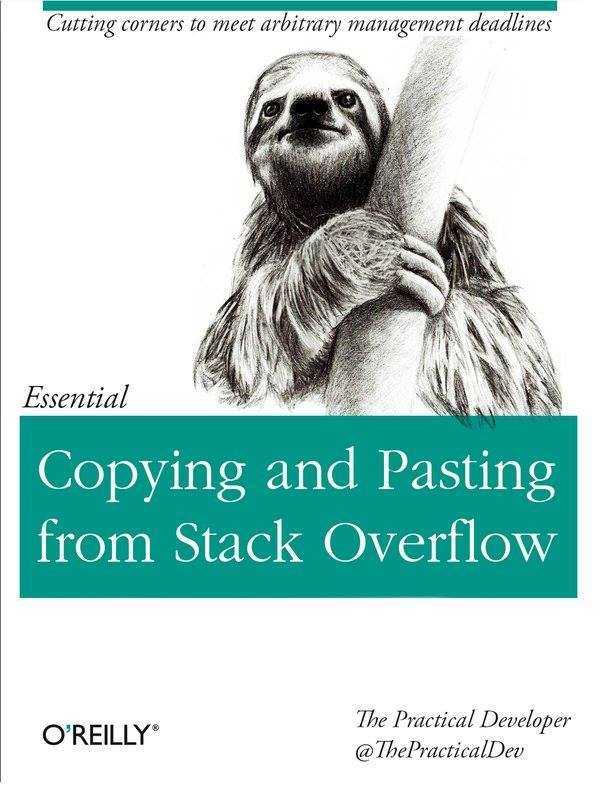
\includegraphics[width=0.8\textwidth]{figures/copypasta.jpg}
    \caption{What's this, another joke?}
    \label{fig:copypasta}
\end{figure}

\section*{Chapter Summary}
In this chapter, we explored:
\begin{itemize}
\item How this book is funded and the importance of supporting creators.
\item The philosophy of open source and its role in this project.
\item Tools and resources to get started.
\item Ethical and practical ways to engage with the content.
\end{itemize}

By understanding these principles, you\textquoteright re not just learning to install tools; you\textquoteright re joining a vibrant community of creators and learners. Welcome to the journey!

\subsection{Cick Me}

Here are some useful links:

\begin{itemize}
    \item \href{https://www.overleaf.com}{Overleaf - Online LaTeX Editor}
    \item \href{https://www.ctan.org}{CTAN - Comprehensive TeX Archive Network}
    \item \href{https://turtletoy.net}{Turtletoy - Generative Art Platform}
    \item \href{https://arxiv.org}{arXiv - Open Access Research Papers}
    \item \href{https://github.com}{GitHub - Code Hosting Platform}
    \item \href{https://numpy.org}{NumPy - Python Library for Scientific Computing}
    \item \href{https://openai.com}{OpenAI - AI Research Organization}
    \item \href{https://projecteuclid.org}{Project Euclid - Mathematics Research}
    \item \href{https://www.math.uwaterloo.ca/~hwolkowi/matrixcookbook.pdf}{The Matrix Cookbook}
    \item \href{https://thebookofshaders.com/}{The Book of Shaders}
    \item \href{https://github.com/beardicus/awesome-plotters}{Plotter tutorials 1}
    \item \href{https://www.generativehut.com/tutorials}{Plotter tutorials 2}

    \item \href{https://oken.do/ggmh4kmj}{Household Goods (Good Store code)}
    \item \href{https://ubereats.com/feed?promoCode=eats-i81xs}{Feed Me (Uber eats code)}
    \item \href{https://www.instagram.com/chromatocosmos/}{Follow Me on IG}
    \item \href{https://www.linkedin.com/in/geoffrey-bradway/}{Follow Me on LinkedIn}
    
\end{itemize}


\chapter{On Games of Chance}
\section{AIs as Association Machines}
\insertmydocument{section}{AI as Association Machines}{}{AI_as_Association_Machines.pdf}


\section{The Law of Large Numbers \cite{davar} and the Central Limit Theorem: Foundations of Probability}

\subsection*{Introduction}
Probability theory provides a structured framework to understand uncertainty and randomness in the natural world. Two cornerstone concepts within this field are the \textit{Law of Large Numbers} (LLN) and the \textit{Central Limit Theorem} (CLT). These theorems, often working in tandem, offer profound insights into the behavior of repeated random experiments, guiding the way we think about statistics and data.

\subsection*{The Law of Large Numbers}
The Law of Large Numbers is an elegant principle that describes the stabilization of sample averages as the number of trials increases. Formally, the LLN states that as the number of independent and identically distributed (i.i.d.) trials of a random variable grows, the sample mean converges to the expected value of the random variable.

\subsection*{Illustration Through Coin Flipping}
Consider flipping a fair coin. The probability of landing heads in a single trial is $0.5$. If we flip the coin a small number of times, we might observe outcomes that deviate from this expectation---for instance, 7 heads in 10 flips. However, as we repeat the experiment thousands of times, the proportion of heads will tend toward $0.5$. This phenomenon is the essence of the LLN: the empirical probability converges to the theoretical probability.

The significance of the LLN is widespread. It underpins fields like insurance and finance, where averages over large populations are used to predict outcomes with remarkable accuracy. By ensuring that sample statistics reflect population parameters, the LLN builds a bridge between theory and observation.

\section*{The Central Limit Theorem}
While the LLN describes the stabilization of averages, the Central Limit Theorem delves deeper into their distribution. The CLT states that, regardless of the underlying distribution of a random variable, the distribution of the sample mean approaches a normal (Gaussian) distribution as the sample size grows, provided the random variable has a finite mean and variance.

\subsection*{Key Features of the CLT}
\begin{itemize}
    \item \textbf{Universality:} The CLT applies to nearly any random variable, irrespective of its original distribution---be it uniform, exponential, or skewed.
    \item \textbf{Shape of the Distribution:} As sample size increases, the shape of the sampling distribution of the mean becomes bell-shaped, centered around the population mean, with a standard deviation proportional to $\frac{\sigma}{\sqrt{n}}$, where $\sigma$ is the population standard deviation and $n$ is the sample size.
\end{itemize}

\subsection*{Example: Rolling Dice}
Imagine rolling a six-sided die. The sum of the outcomes for a small number of rolls might not resemble any familiar distribution. But if we repeatedly roll the die and calculate the average outcome over increasingly large groups, the distribution of these averages will approximate a normal curve, centered at the expected value of $3.5$.

\section*{Practical Applications and Interplay}
The combination of the LLN and CLT is foundational to modern statistical inference. Together, they justify the use of sample statistics to estimate population parameters and assess uncertainties:

\begin{itemize}
    \item \textbf{Sampling and Estimation:} The LLN ensures that sample averages provide reliable estimates of population means, while the CLT allows us to calculate confidence intervals and make probabilistic predictions.
    \item \textbf{Predictive Models:} In machine learning and artificial intelligence, these theorems underlie methods for training models and evaluating their performance over large datasets.
    \item \textbf{Finance and Risk Management:} Financial analysts rely on these principles to model stock returns, assess risks, and optimize portfolios.
\end{itemize}

\section*{A Philosophical Reflection}
Both the LLN and CLT highlight the surprising order embedded within randomness. They demonstrate that even in the face of individual uncertainty, patterns emerge when viewed at scale. This interplay between chaos and structure is not just a mathematical truth---it resonates with broader themes in science and philosophy.

\section*{Conclusion}
In summary, the Law of Large Numbers and the Central Limit Theorem are more than mathematical theorems; they are lenses through which we perceive and interpret randomness. Their implications ripple across disciplines, shaping how we measure, predict, and reason about the world.

\insertmydocument{section}{AI as Association Machines}{}{cah-print.pdf}

\documentclass[12pt]{article}
\usepackage{amsmath, amssymb, graphicx, hyperref}
\usepackage{amsfonts}
\usepackage[mathletters]{ucs}
\usepackage{geometry}
\geometry{a4paper, margin=1in}
\title{An Exploration of Light, Optics, Halftones, and Generative Art}
\author{}
\date{}

\begin{document}
\maketitle

\section*{Introduction}
Light and its interaction with matter form the foundation of both artistic expression and scientific inquiry. From the intricate physics of optics to the computational techniques of halftones and image replication, the interplay of light, color, and geometry reveals profound insights into our understanding of the visual world. This essay introduces the central themes of this project, connecting the scientific and artistic domains to explore how ideas like CMYK versus RGB, moir\'{e} patterns, and Sobel-filtered gradient matching are utilized in generative art.

\section*{The Science of Light and Optics}
Light, as both wave and particle, has captivated scientists for centuries. Optics, the study of light's behavior, provides tools to understand phenomena such as reflection, refraction, and diffraction. These principles are pivotal in modern technology, from lasers to lenses. The ability to manipulate light also underpins artistic techniques, allowing the creation of depth, contrast, and texture in visual representations.

\subsection*{Color Spaces: RGB and CMYK}
Color is a critical aspect of visual art and design, and its representation involves distinct mathematical frameworks. RGB (Red, Green, Blue) and CMYK (Cyan, Magenta, Yellow, Key/Black) are two primary color spaces used in digital screens and print, respectively. RGB combines emitted light to create colors, relying on additive color mixing. CMYK, in contrast, subtracts light using inks or pigments, making it better suited for physical media. Understanding these systems is vital for converting designs between digital and print formats without loss of fidelity.

\section*{Halftones and Moir\'{e} Patterns}
Halftones approximate continuous tones in printed images by using dots of varying sizes and densities. This method exploits the human eye's tendency to blend small details into a coherent whole. However, when overlapping halftone patterns occur, they may produce moir\'{e} patterns: interference effects that result in unexpected visual artifacts. While often undesirable, these patterns can also inspire creative exploration in generative art.

\section*{Generative Art and Gradient Matching}
Generative art bridges the gap between technology and creativity, using algorithms to produce designs. One innovative approach involves Sobel filters, which detect image gradients by emphasizing edges. By employing stochastic gradient descent (SGD), a blank grid can deform to match these gradients, effectively replicating an image's structure. This technique highlights the intersection of mathematics, computation, and aesthetics, enabling artists to push boundaries and reimagine traditional concepts.

\section*{Philosophical Reflection}
As George Berkeley once said, \emph{\textquotedblleft To be is to be perceived.\textquotedblright} This perspective connects deeply with the themes of light and perception explored in this project. The notion underscores how our understanding of the visual world is inherently tied to how it is observed and interpreted.

\href{https://www.youtube.com/watch?v=idl8TvI-0iw}{Click here for a related video discussion on this topic.}

\section*{Integrating Science and Art}
The project's files showcase various explorations into these themes:

\begin{itemize}
    \item The Jupyter notebook delves into procedural designs, employing libraries such as Shapely and NumPy to generate geometrical patterns.
    \item The SVG file represents stippled designs, demonstrating the application of computational geometry in art.
    \item Photographic examples illustrate how light and optics influence real-world visuals, setting the stage for generative reinterpretations.
\end{itemize}

\section*{The Lebesgue Dominated Convergence Theorem: A High-Level Overview}
The Lebesgue Dominated Convergence Theorem (LDCT) is a cornerstone of measure theory and integral calculus. It provides conditions under which the limit of an integral can be exchanged with the integral of a limit. This is particularly useful in mathematical analysis, probability theory, and applied fields like physics and engineering.

In essence, LDCT states that if a sequence of functions \(f_n\) converges pointwise to a function \(f\), and there exists a dominating function \(g\) such that \(|f_n(x)| \leq g(x)\) for all \(n\) and \(x\), and \(g\) is integrable (i.e., \(\int g < \infty\)), then:
\[
\lim_{n \to \infty} \int f_n(x) \, dx = \int \lim_{n \to \infty} f_n(x) \, dx.
\]

This theorem elegantly combines the concepts of convergence, domination, and integration, ensuring the transition from pointwise to integral limits is valid. Its applications range from simplifying complex integrals to proving convergence results in stochastic processes and partial differential equations.

\end{document}

\section*{Conclusion}
This project marries scientific principles with artistic creativity, exploring how light, color, and geometry shape our perception and expression. By examining the connections between halftones, color spaces, and computational techniques, we gain deeper appreciation for the shared language of art and science, rooted in the universal interplay of light and shadow.

\end{document}


\section{Optickal References}

\insertmydocument{section}{Opticks in Action}{}{production-Copy1.pdf}

\begin{figure}
        \centering
        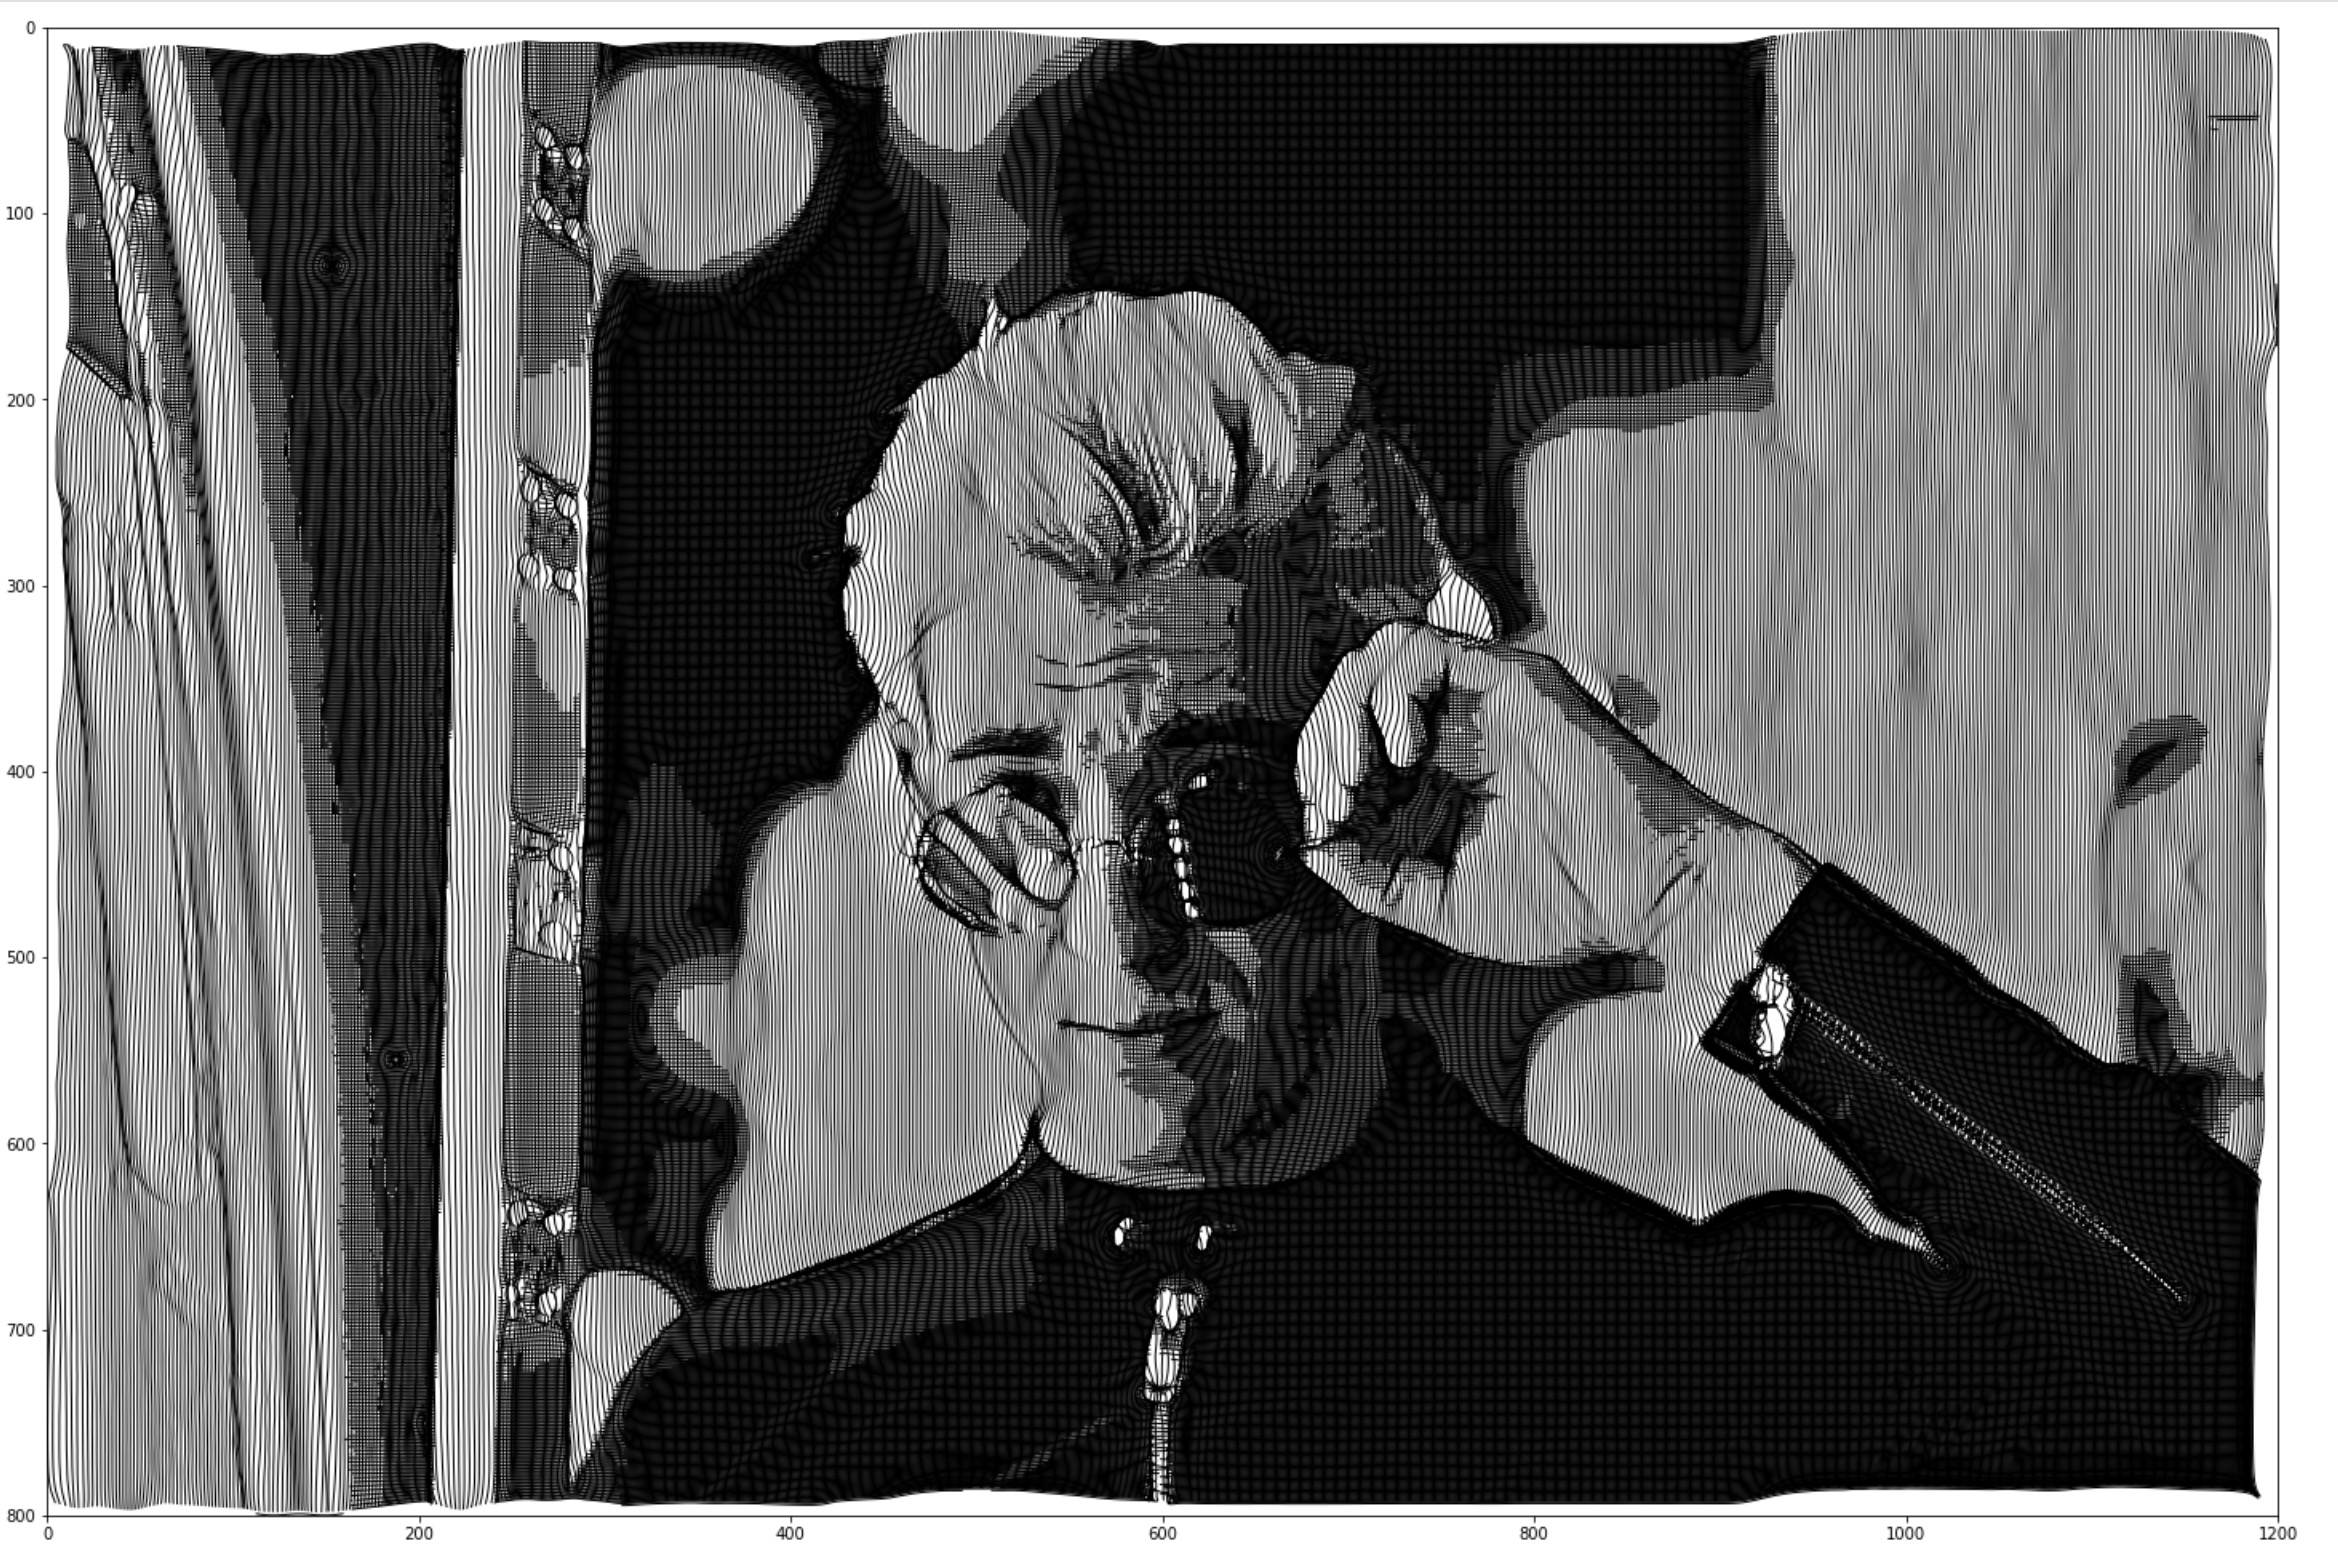
\includegraphics[width=0.8\textwidth]{figures/ofig/IMG_0925.jpg}
    \end{figure}

\begin{figure}
        \centering
        \includegraphics[width=0.8\textwidth]{figures/ofig/P1100533.JPG}
    \end{figure}

\begin{figure}
        \centering
        \includegraphics[width=0.8\textwidth]{figures/ofig/P1590969.JPG}
    \end{figure}

\begin{figure}
        \centering
        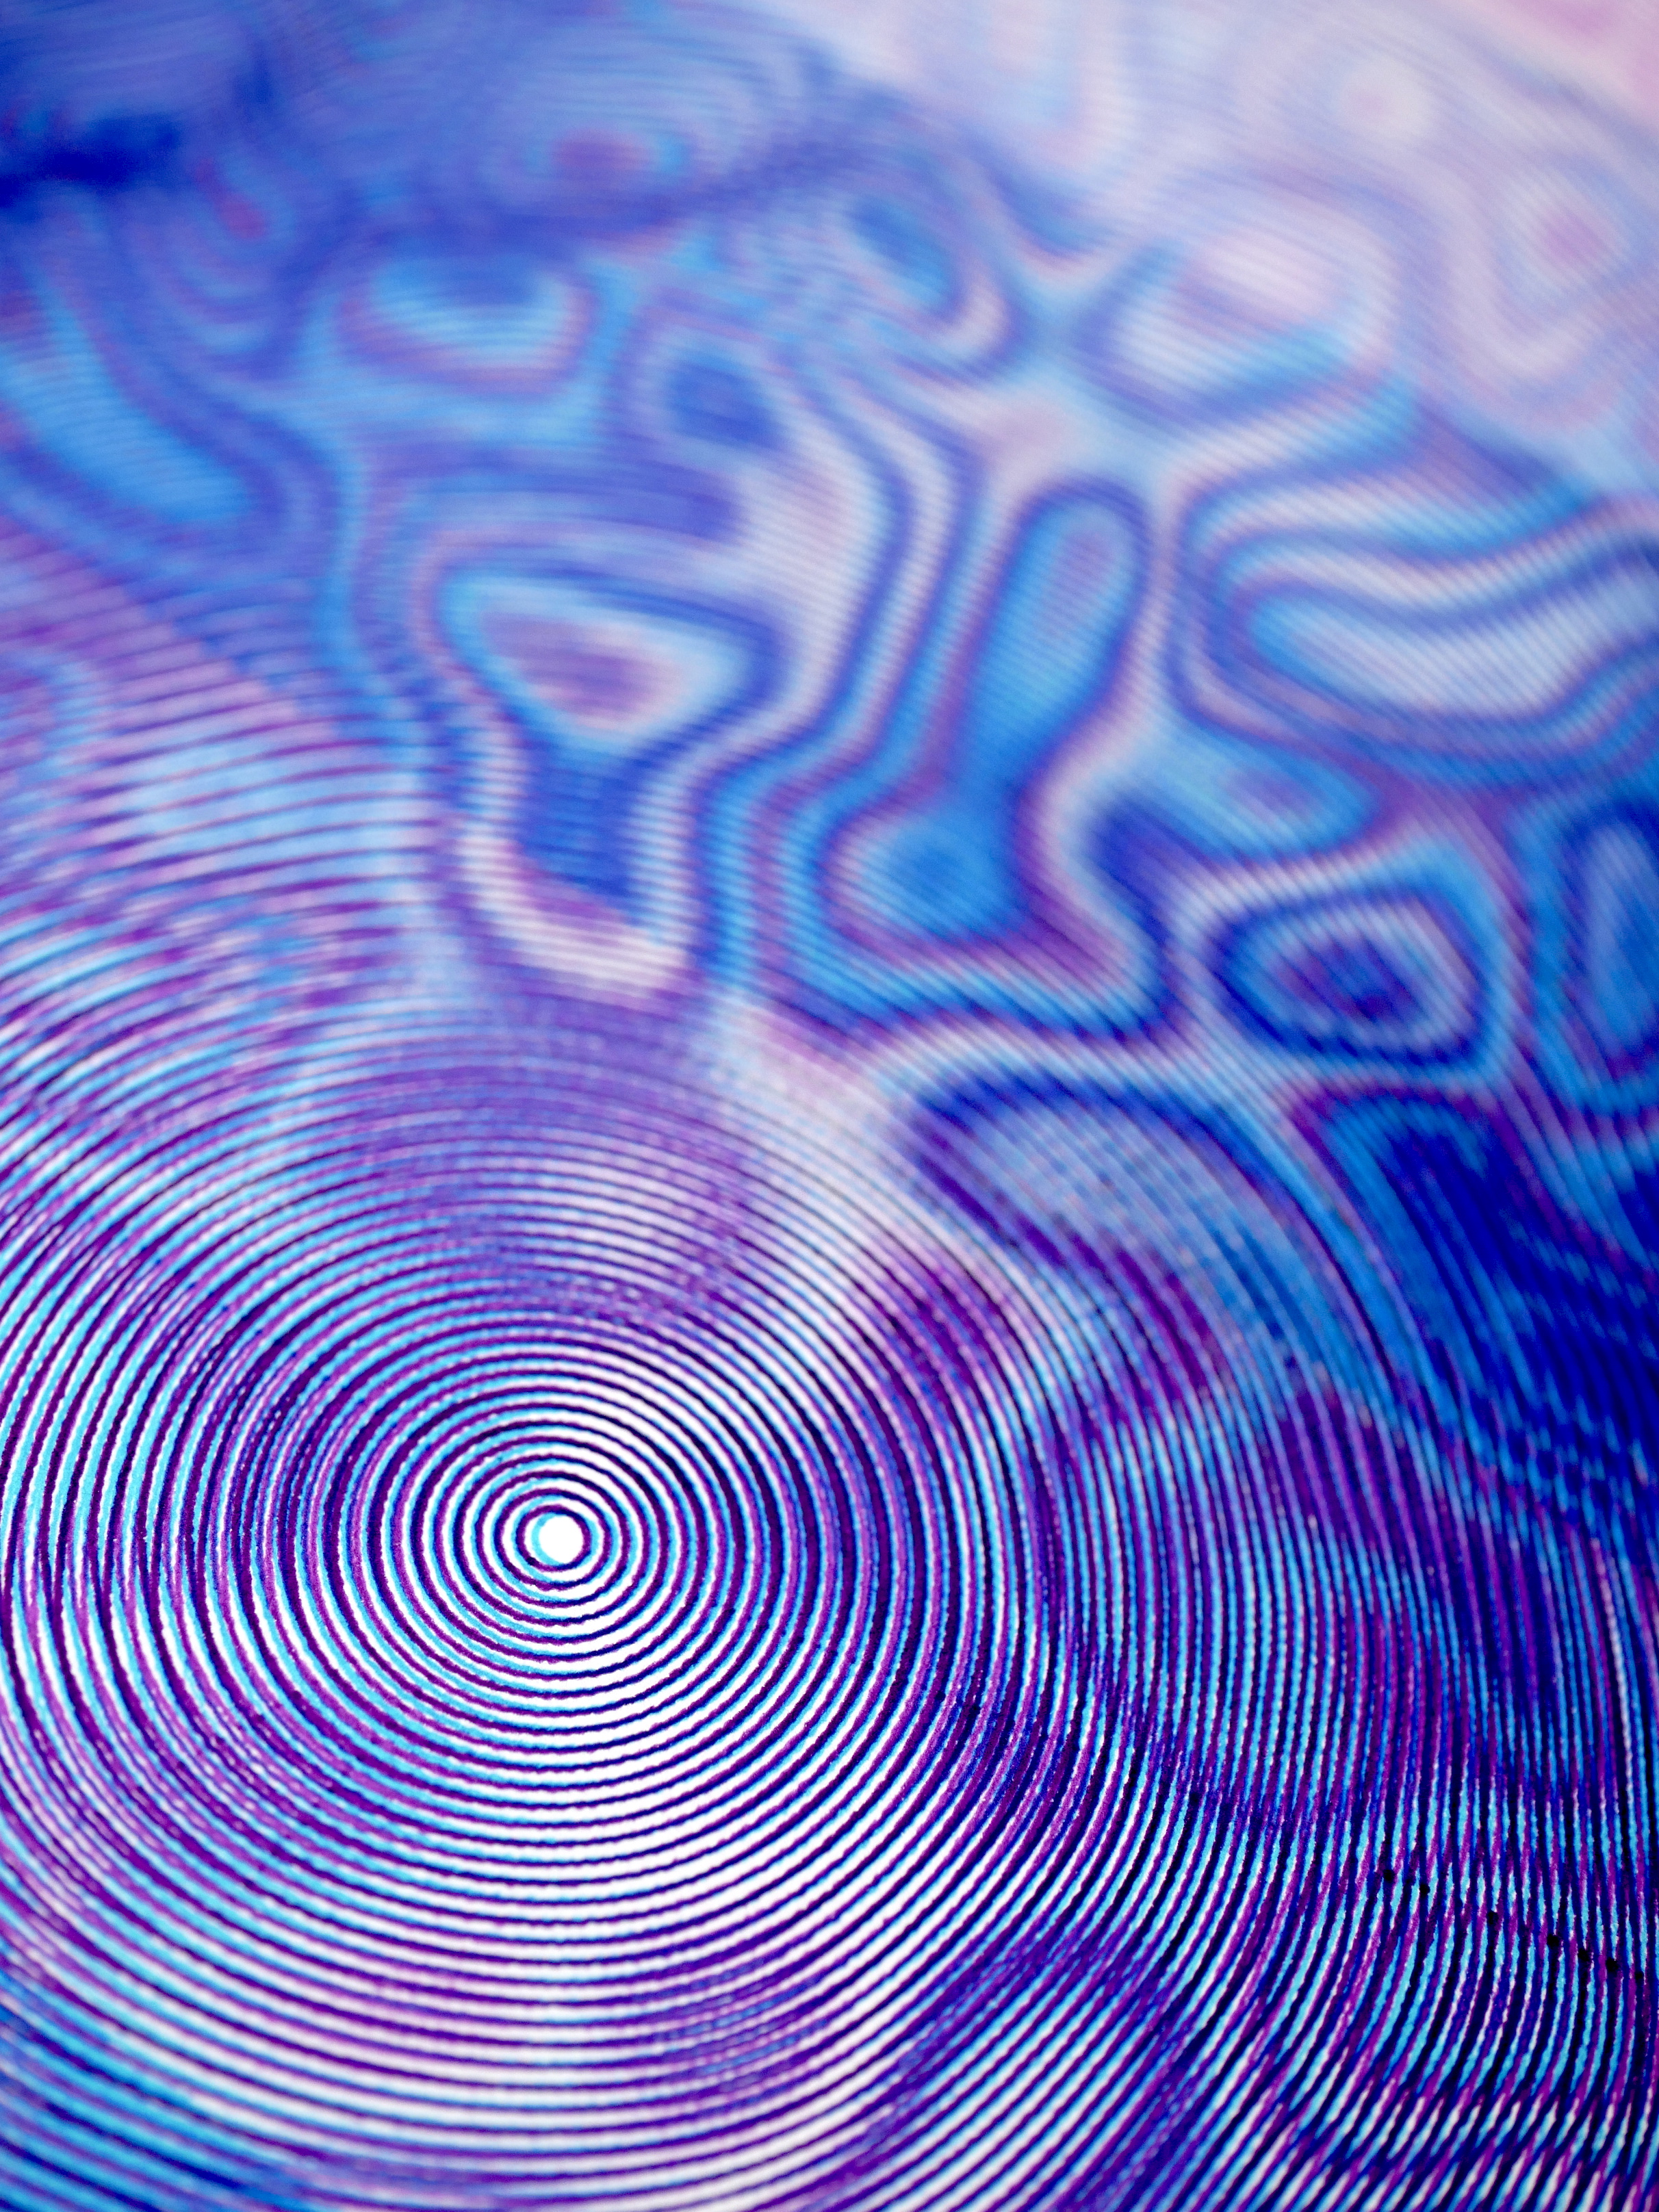
\includegraphics[width=0.8\textwidth]{figures/ofig/P1600032.JPG}
    \end{figure}

\begin{figure}
        \centering
        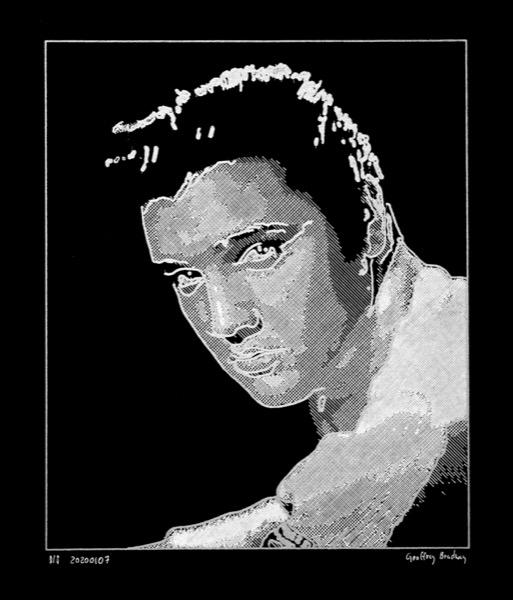
\includegraphics[width=0.8\textwidth]{figures/ofig/P1770280.JPG}
    \end{figure}

\begin{figure}
        \centering
        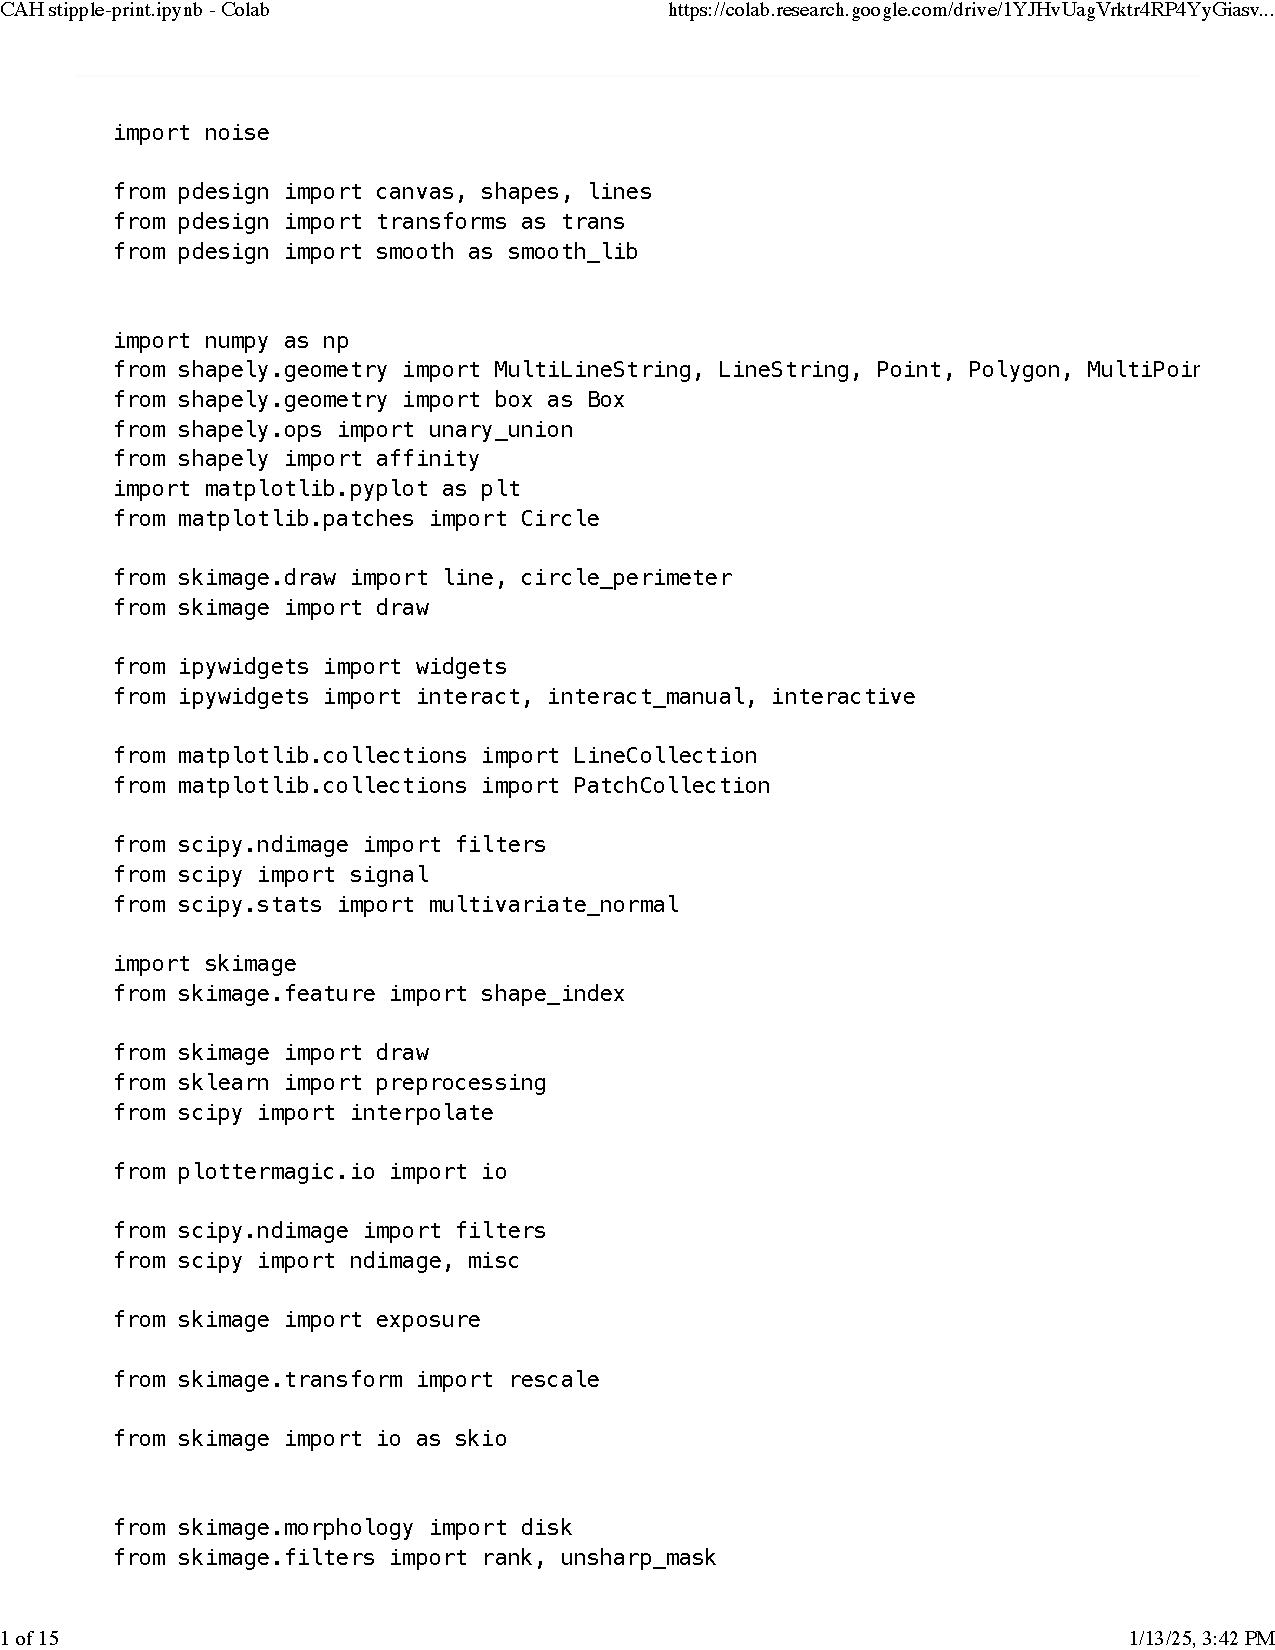
\includegraphics[width=0.8\textwidth]{figures/ofig/cah-email-print.pdf}
    \end{figure}

\begin{figure}
        \centering
        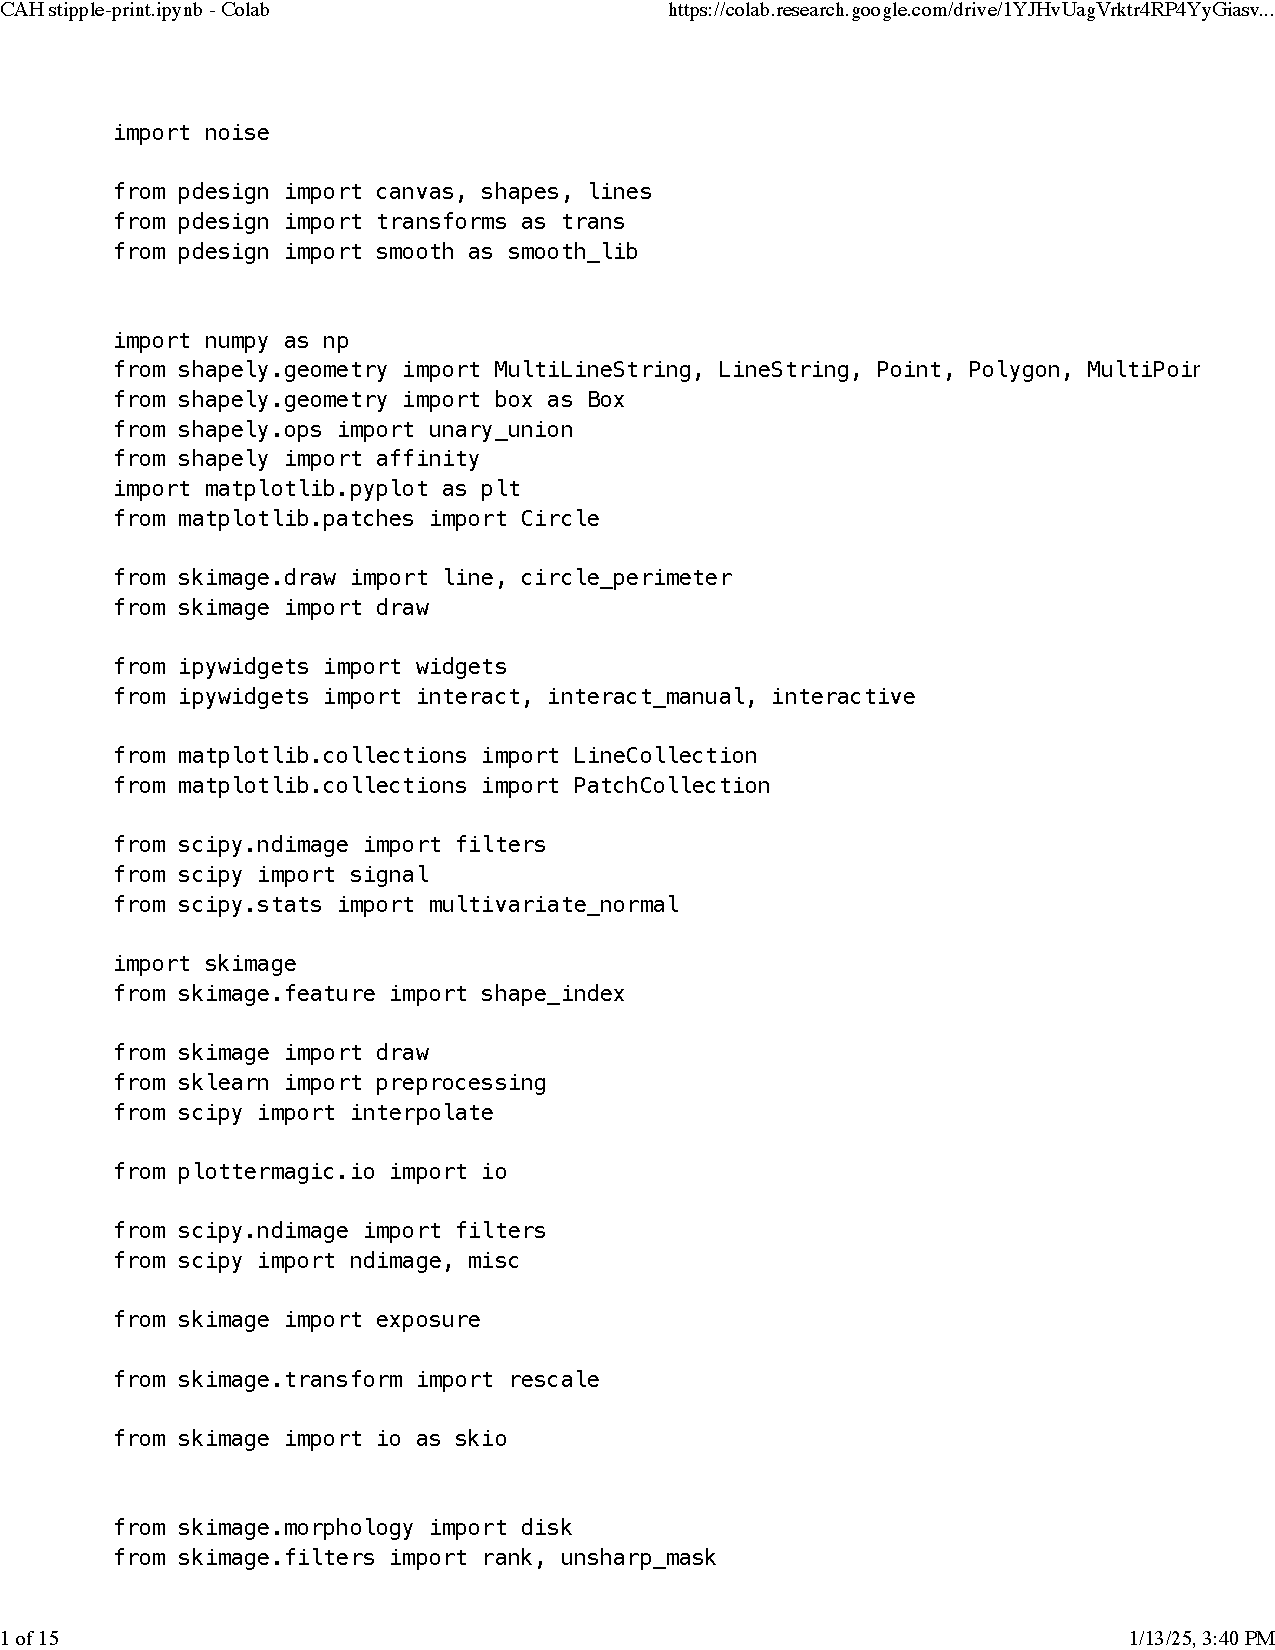
\includegraphics[width=0.8\textwidth]{figures/ofig/cah-print.pdf}
    \end{figure}

\begin{figure}
        \centering
        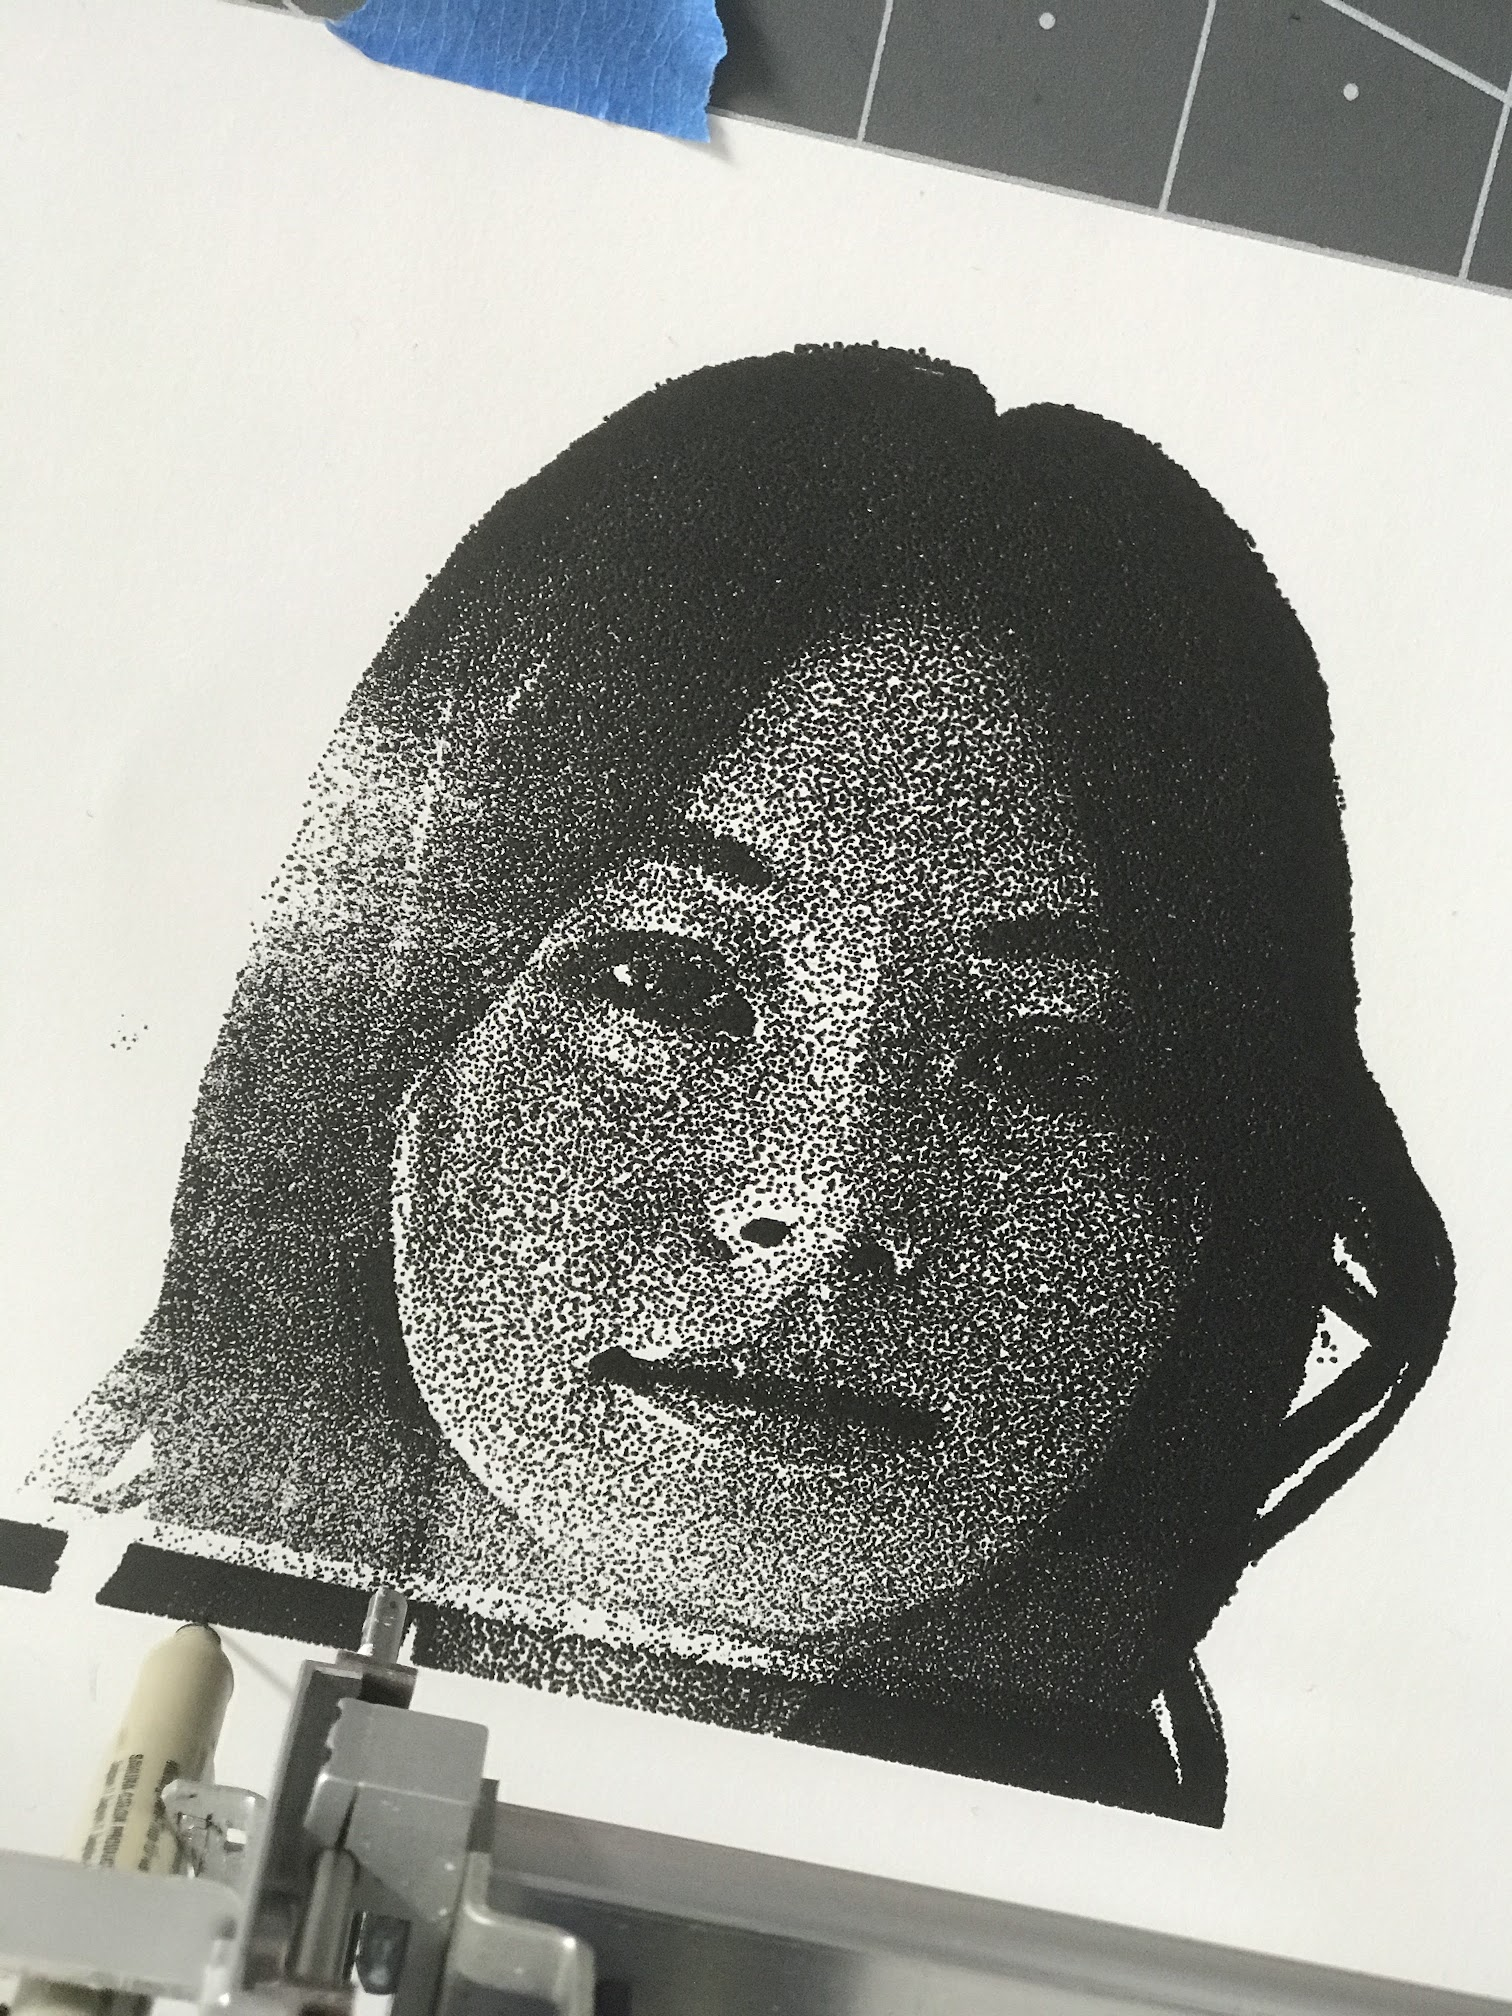
\includegraphics[width=0.8\textwidth]{figures/ofig/marie.jpg}
    \end{figure}

\begin{figure}
        \centering
        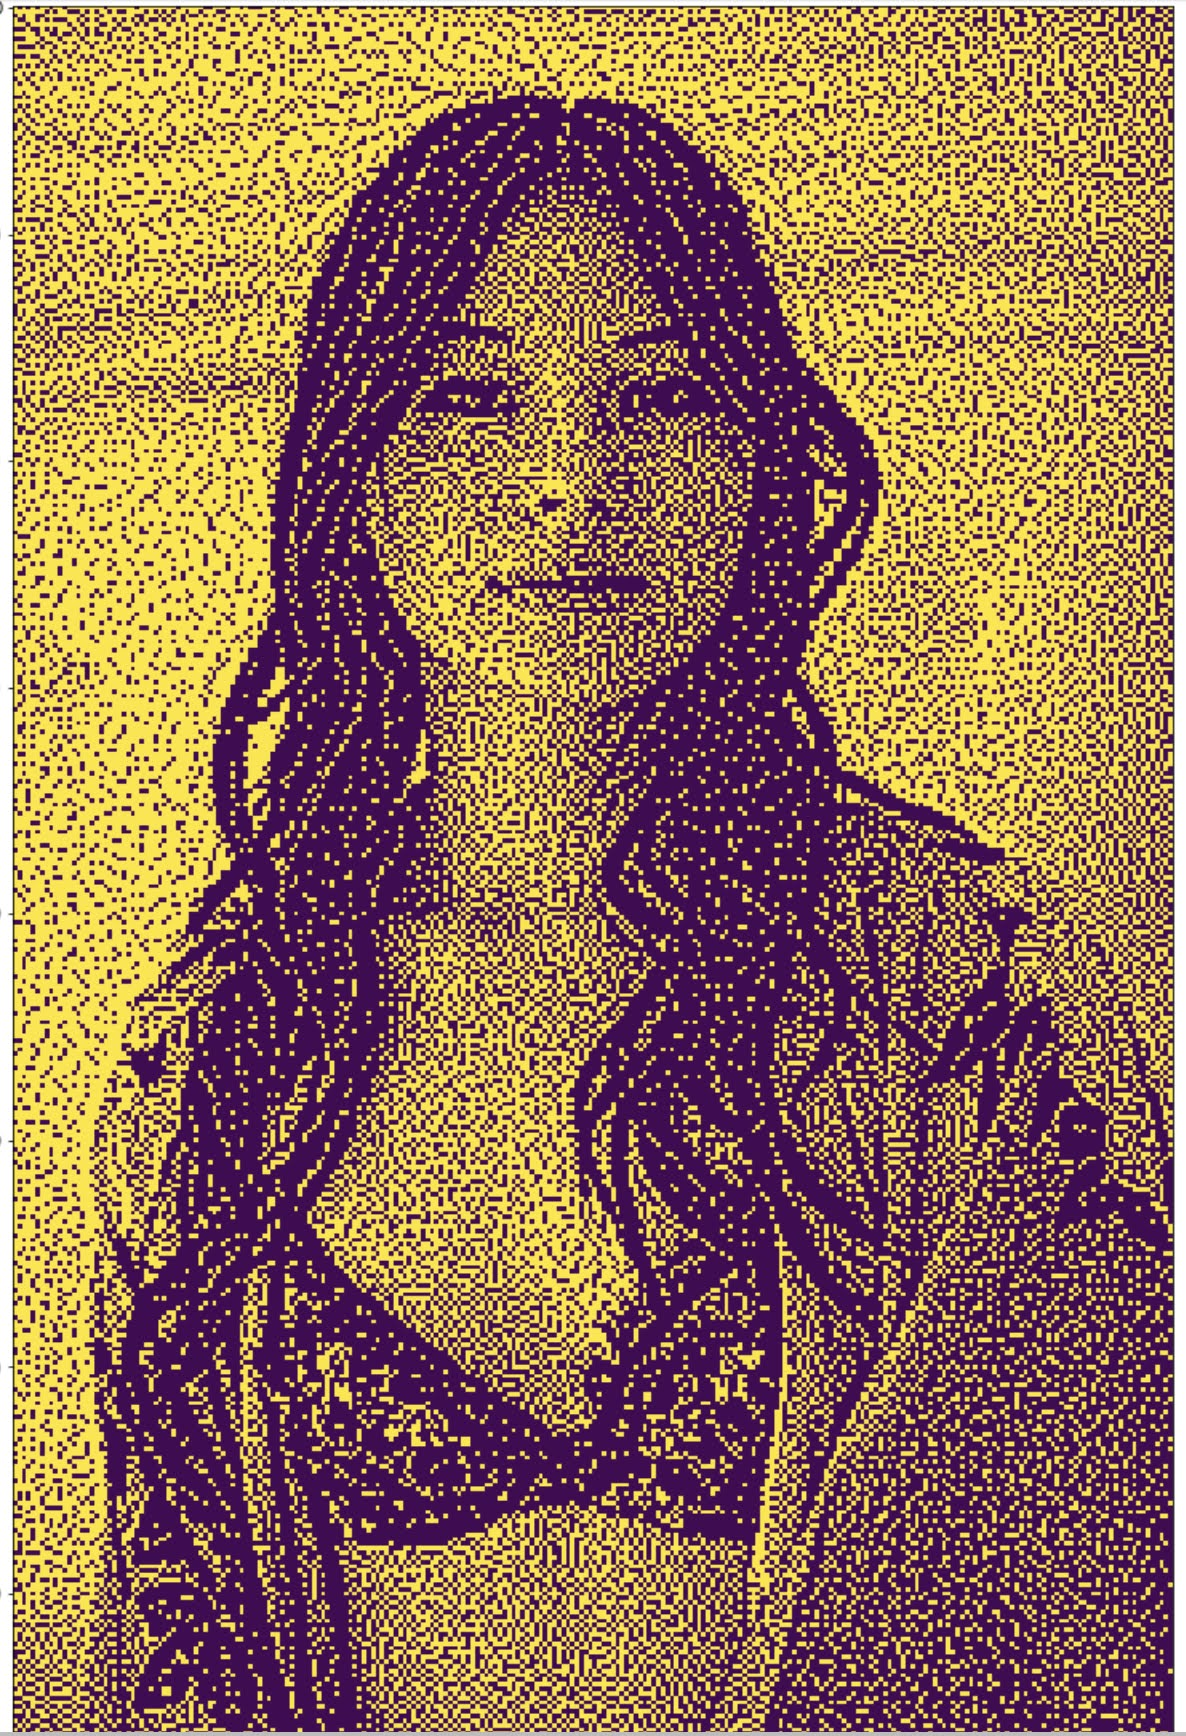
\includegraphics[width=0.8\textwidth]{figures/ofig/marie8bit.jpg}
    \end{figure}

\begin{figure}
        \centering
        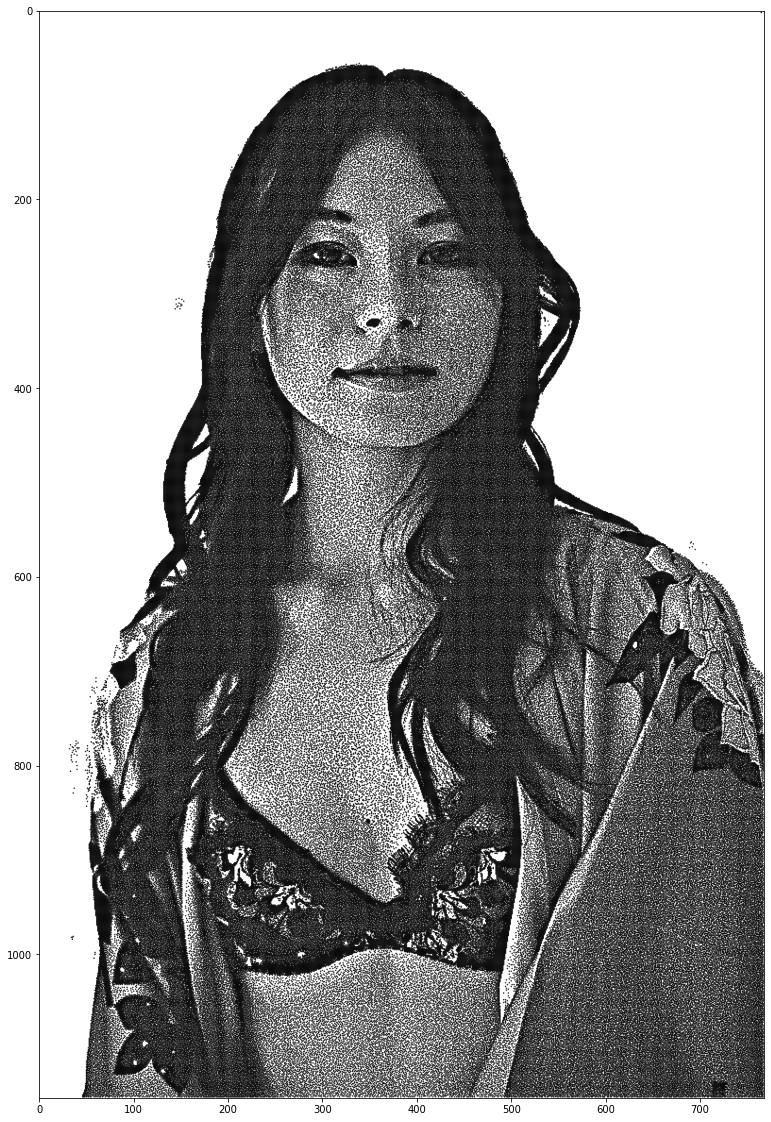
\includegraphics[width=0.8\textwidth]{figures/ofig/marie_nice_render.png}
    \end{figure}

\begin{figure}
        \centering
        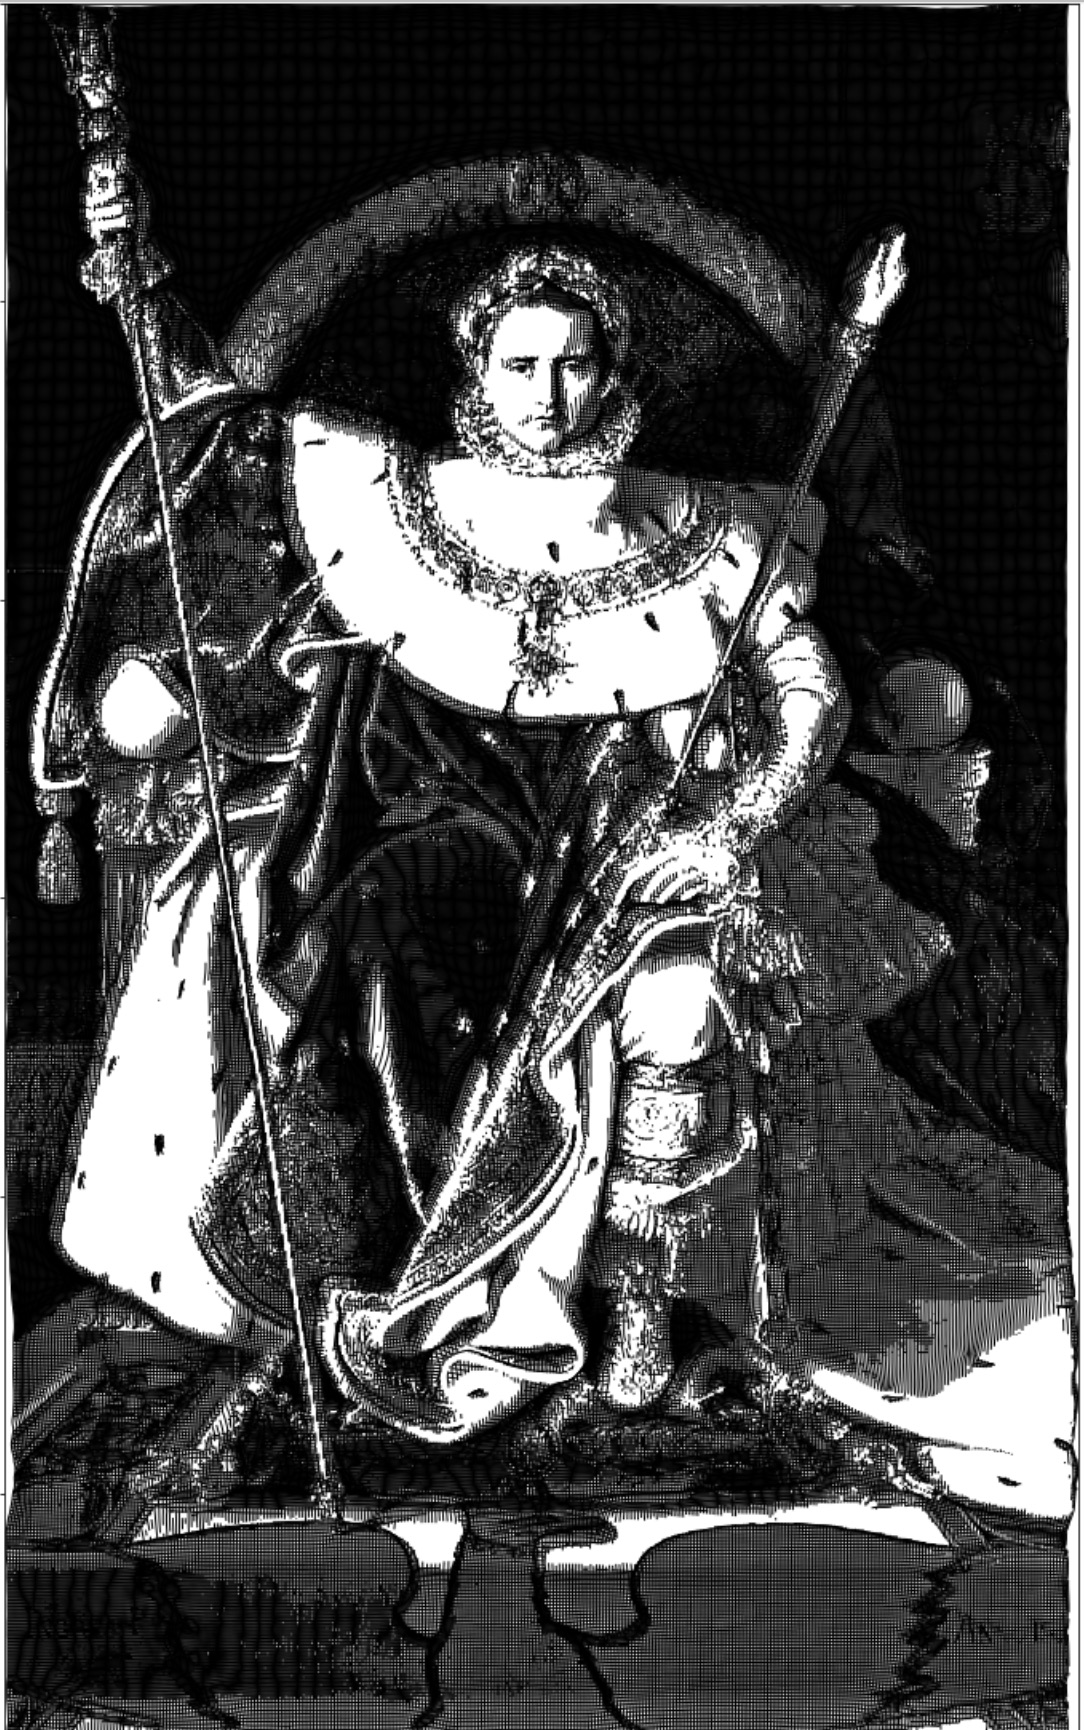
\includegraphics[width=0.8\textwidth]{figures/ofig/napolean_nice_render.jpg}
    \end{figure}


\chapter{Ways of Seeing}

\chapter{Some Seeds for Gardening}

Here are some useful links:

\begin{itemize}
    \item \href{https://github.com/zoso95/lsystems}{L Systems that adapt over time}
    \item \href{https://github.com/zoso95/genetic-algorithm-fractals}{Genetic Algorithm Fractals}
    \item \href{https://github.com/zoso95/3d-object-parsing}{3d Object Parsing}
    \item \href{https://github.com/zoso95/freetimescheduler}{Free Time Scheduler}
\end{itemize}


\chapter{Laplace}
\section*{Laplacian Pyramid Blending: A High-Level Overview}
Laplacian Pyramid Blending is a technique in image processing used to seamlessly combine two images. By leveraging multiscale image representations, the method ensures smooth transitions between blended regions, preserving both detail and context.

\subsection*{Conceptual Framework}
The process relies on constructing multiscale representations of the images to be blended. This involves two key pyramids:

\begin{itemize}
    \item \textbf{Gaussian Pyramid:} A series of increasingly blurred and downsampled versions of the image, capturing low-frequency information.
    \item \textbf{Laplacian Pyramid:} Obtained by subtracting consecutive levels of the Gaussian pyramid, it encodes band-pass frequency information.
\end{itemize}

Blending is achieved by combining the Laplacian pyramids of the two images, guided by a blending mask. The mask, also represented as a Gaussian pyramid, determines the contribution of each image at different scales. Finally, the blended Laplacian pyramid is collapsed back to reconstruct the final image.

\subsection*{Algorithm Steps}
\begin{enumerate}
    \item \textbf{Construct Gaussian Pyramids:} Generate Gaussian pyramids for the input images and the blending mask.
    \item \textbf{Construct Laplacian Pyramids:} Build Laplacian pyramids for the input images by subtracting adjacent levels of their Gaussian pyramids.
    \item \textbf{Blend Pyramids:} Combine the Laplacian pyramids of the two images at each level using the Gaussian pyramid of the mask as weights.
    \item \textbf{Reconstruct the Image:} Collapse the blended Laplacian pyramid to obtain the final output image.
\end{enumerate}

\subsection*{Implementation Example}
The Python implementation below demonstrates Laplacian Pyramid Blending using the \texttt{skimage} library:

\begin{verbatim}
from skimage.transform import pyramids
from skimage.filters import gaussian
import numpy as np

def laplacian_pyramid_blending(img_a, img_b, mask, n_layers=4):
    g1 = [e for e in pyramids.pyramid_gaussian(img_a, max_layer=n_layers)]
    g2 = [e for e in pyramids.pyramid_gaussian(img_b, max_layer=n_layers)]
    gm = [e for e in pyramids.pyramid_gaussian(mask, max_layer=n_layers)]

    l1 = [g1[i] - pyramids.transform.rescale(g1[i+1], 2) for i in range(n_layers-1)]
    l2 = [g2[i] - pyramids.transform.rescale(g2[i+1], 2) for i in range(n_layers-1)]

    blended_pyramid = [l1[i] * gm[i] + l2[i] * (1 - gm[i]) for i in range(n_layers-1)]
    blended_pyramid.append(gm[-1] * g1[-1] + (1 - gm[-1]) * g2[-1])

    blended_img = blended_pyramid[-1]
    for i in range(n_layers-2, -1, -1):
        blended_img = pyramids.transform.rescale(blended_img, 2) + blended_pyramid[i]

    return blended_img
\end{verbatim}

\subsection*{Applications}
\begin{itemize}
    \item \textbf{Panorama Stitching:} Seamlessly blending overlapping regions of images.
    \item \textbf{Photo Compositing:} Combining features of two or more images into a single coherent image.
    \item \textbf{Special Effects:} Creating visually appealing transitions and effects in media production.
\end{itemize}

\subsection*{Visualization}
Below is an example result showing the seamless blending of two images using a triangular mask:

\begin{verbatim}
# Visualization code example
mask = np.zeros_like(img_a)
tri_x, tri_y = draw.polygon([0, 0, img_a.shape[0]], [0, img_a.shape[1], img_a.shape[1]])
mask[tri_x, tri_y] = 1
mask = gaussian(mask, sigma=20)

blended_image = laplacian_pyramid_blending(img_a, img_b, mask)
plt.imshow(blended_image, cmap='gray')
\end{verbatim}

\section*{Conclusion}
Laplacian Pyramid Blending showcases the power of multiscale image processing in achieving smooth and realistic transitions between blended regions. Its elegance lies in the combination of mathematical theory and practical implementation, making it a cornerstone in image processing and computational photography.

\section{Laplace Code References}
\insertmydocument{section}{Pyramid Blending}{}{blend.pdf}

\begin{figure}
        \centering
        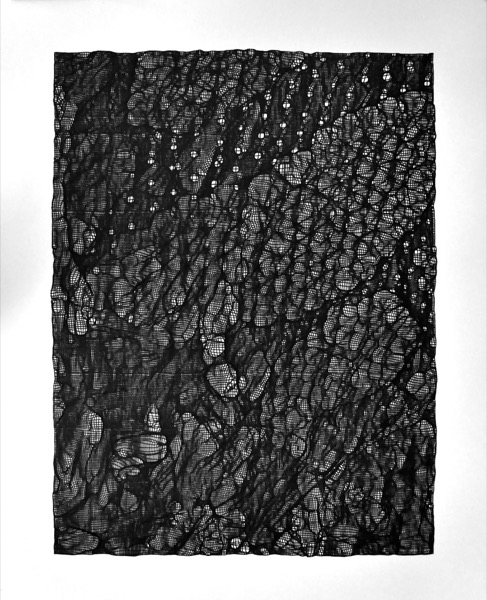
\includegraphics[width=0.8\textwidth]{figures/ofig/snake.JPG}
    \end{figure}


%\insertmydocument{chapter}{Newton's Method}{}{chapters/newton}
\chapter{Newtons Method}
\section*{Newton's Method: A High-Level Overview}
Newton's Method, also known as the Newton-Raphson method, is a powerful iterative technique for finding approximations to the roots of a real-valued function \(f(x)\). Its widespread use in numerical analysis stems from its simplicity, efficiency, and broad applicability.

At its core, Newton's Method leverages the tangent line approximation of a function to iteratively refine guesses for the root. Starting from an initial guess \(x_0\), subsequent approximations are computed using the formula:
\[
    x_{n+1} = x_n - \frac{f(x_n)}{f'(x_n)},
\]
where \(f'(x_n)\) is the derivative of \(f(x)\) evaluated at \(x_n\). The method assumes that \(f(x)\) is differentiable and that \(f'(x_n) \neq 0\).

\subsection*{Applications and Insights}
Newton's Method is employed across various fields, from engineering to computational physics. It is particularly useful when solving nonlinear equations, optimizing functions, and approximating solutions to differential equations. While highly effective under suitable conditions, the method requires careful handling due to potential pitfalls such as divergence or convergence to local extrema instead of the desired root.

\section*{An Iconic Example: The Fast Inverse Square Root}
The Fast Inverse Square Root (\texttt{Q\_rsqrt}) algorithm is a celebrated application of numerical approximation, famously used in graphics engines like the original Quake engine. This algorithm computes \(1 / \sqrt{x}\) with remarkable speed, leveraging bit-level manipulation and Newton's Method for refinement.

Below is the original implementation of the algorithm in C:

\begin{verbatim}
float Q_rsqrt( float number )
{
    long i;                     // Integer representation of the float
    float x2, y;                // Variables for intermediate results
    const float threehalfs = 1.5F; // Constant multiplier

    x2 = number * 0.5F;         // Half of the input number
    y  = number;                // Initial guess for the output
    i  = * ( long * ) &y;       // Evil floating point bit-level hacking
    i  = 0x5f3759df - ( i >> 1 ); // What the fuck?
    y  = * ( float * ) &i;      // Reinterpret as float
    y  = y * ( threehalfs - ( x2 * y * y ) ); // 1st iteration
    // y  = y * ( threehalfs - ( x2 * y * y ) ); // 2nd iteration, optional

    return y;
}
\end{verbatim}

\subsection*{Analysis and Commentary}
This code combines low-level bitwise operations with Newton's Method to achieve rapid convergence. The initial guess \(y\) is obtained using a clever bitwise trick, and the iterative step refines the approximation. The comment \texttt{What the fuck?} humorously underscores the ingenuity and obscurity of the magic constant \texttt{0x5f3759df}.

Despite its age, \texttt{Q\_rsqrt} remains a testament to the intersection of mathematical theory and computational creativity. Modern applications may favor accuracy over speed, but the algorithm continues to inspire generations of programmers and mathematicians.

\section*{Conclusion}
Newton's Method and its derivatives, like the Fast Inverse Square Root, illustrate the elegance and practicality of numerical approximation. By blending analytical insights with computational efficiency, these methods enable solutions to complex problems across diverse domains, showcasing the timeless utility of mathematics.

\insertmydocument{section}{Euler's Approximation Code}{}{glitchy_hourglass.pdf}

\section{Euler's Approximation Images}

\begin{figure}
        \centering
        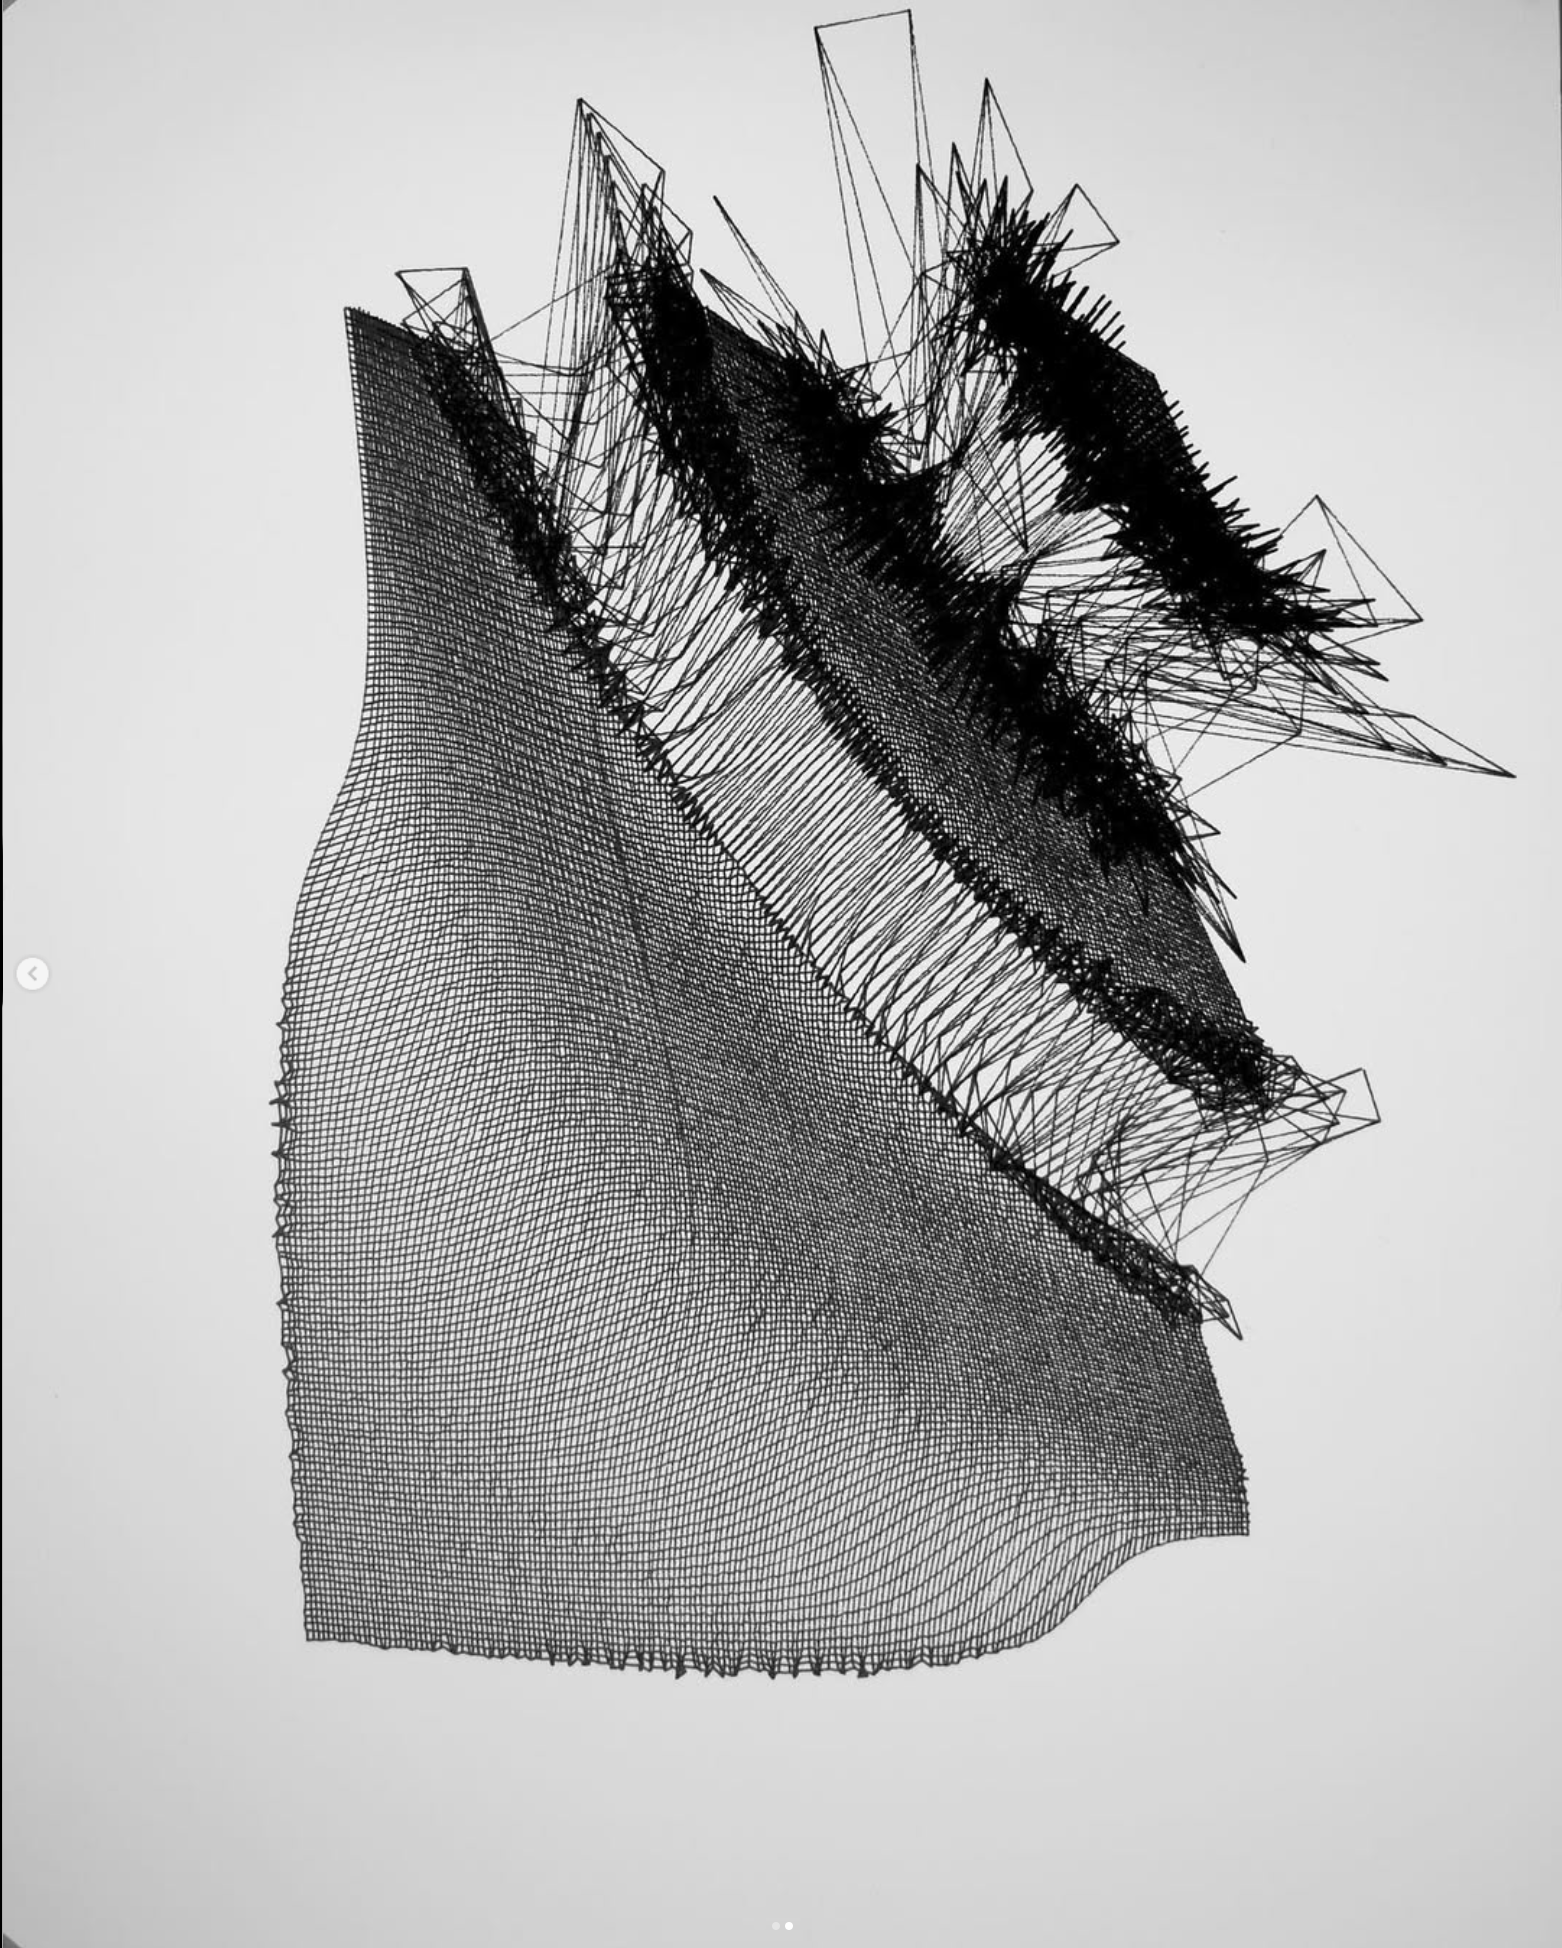
\includegraphics[width=0.8\textwidth]{figures/ofig/Screenshot 2025-01-13 at 4.56.51 PM.png}
    \end{figure}

\chapter{Q-Learning}
\insertmydocument{section}{Masters Project}{}{masters.pdf}

\chapter{The White Paper}
\insertmydocument{section}{Numerai}{}{whitepaper.pdf}

\chapter{The Dinosaur Chapter}
\section{Farmer Labs}
\insertmydocument{subsection}{USet Grant}{}{USETposter.pdf}
\insertmydocument{subsection}{Falcarius}{I have been told those 3d printed turtle shells have made it to a muesum}{FalcariusFinalPaper.pdf}

\section{Dig with Jim Kirkland}

\begin{figure}
    \centering
    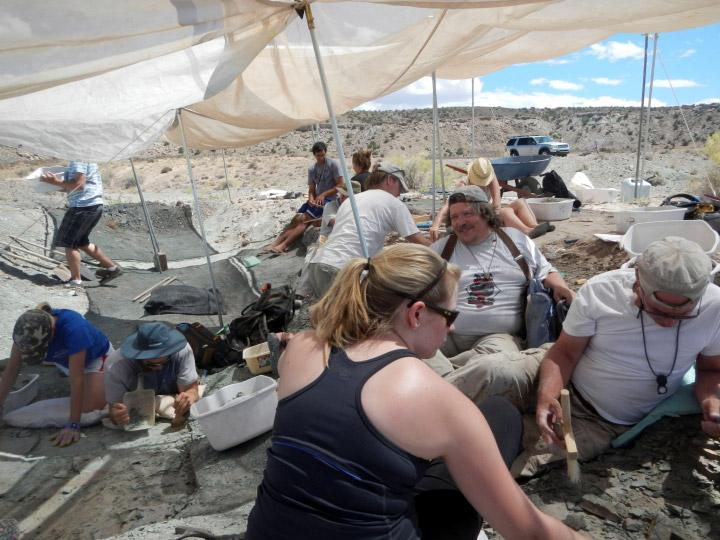
\includegraphics[width=0.8\textwidth]{figures/dig.jpg}
\end{figure}

\begin{figure}
    \centering
    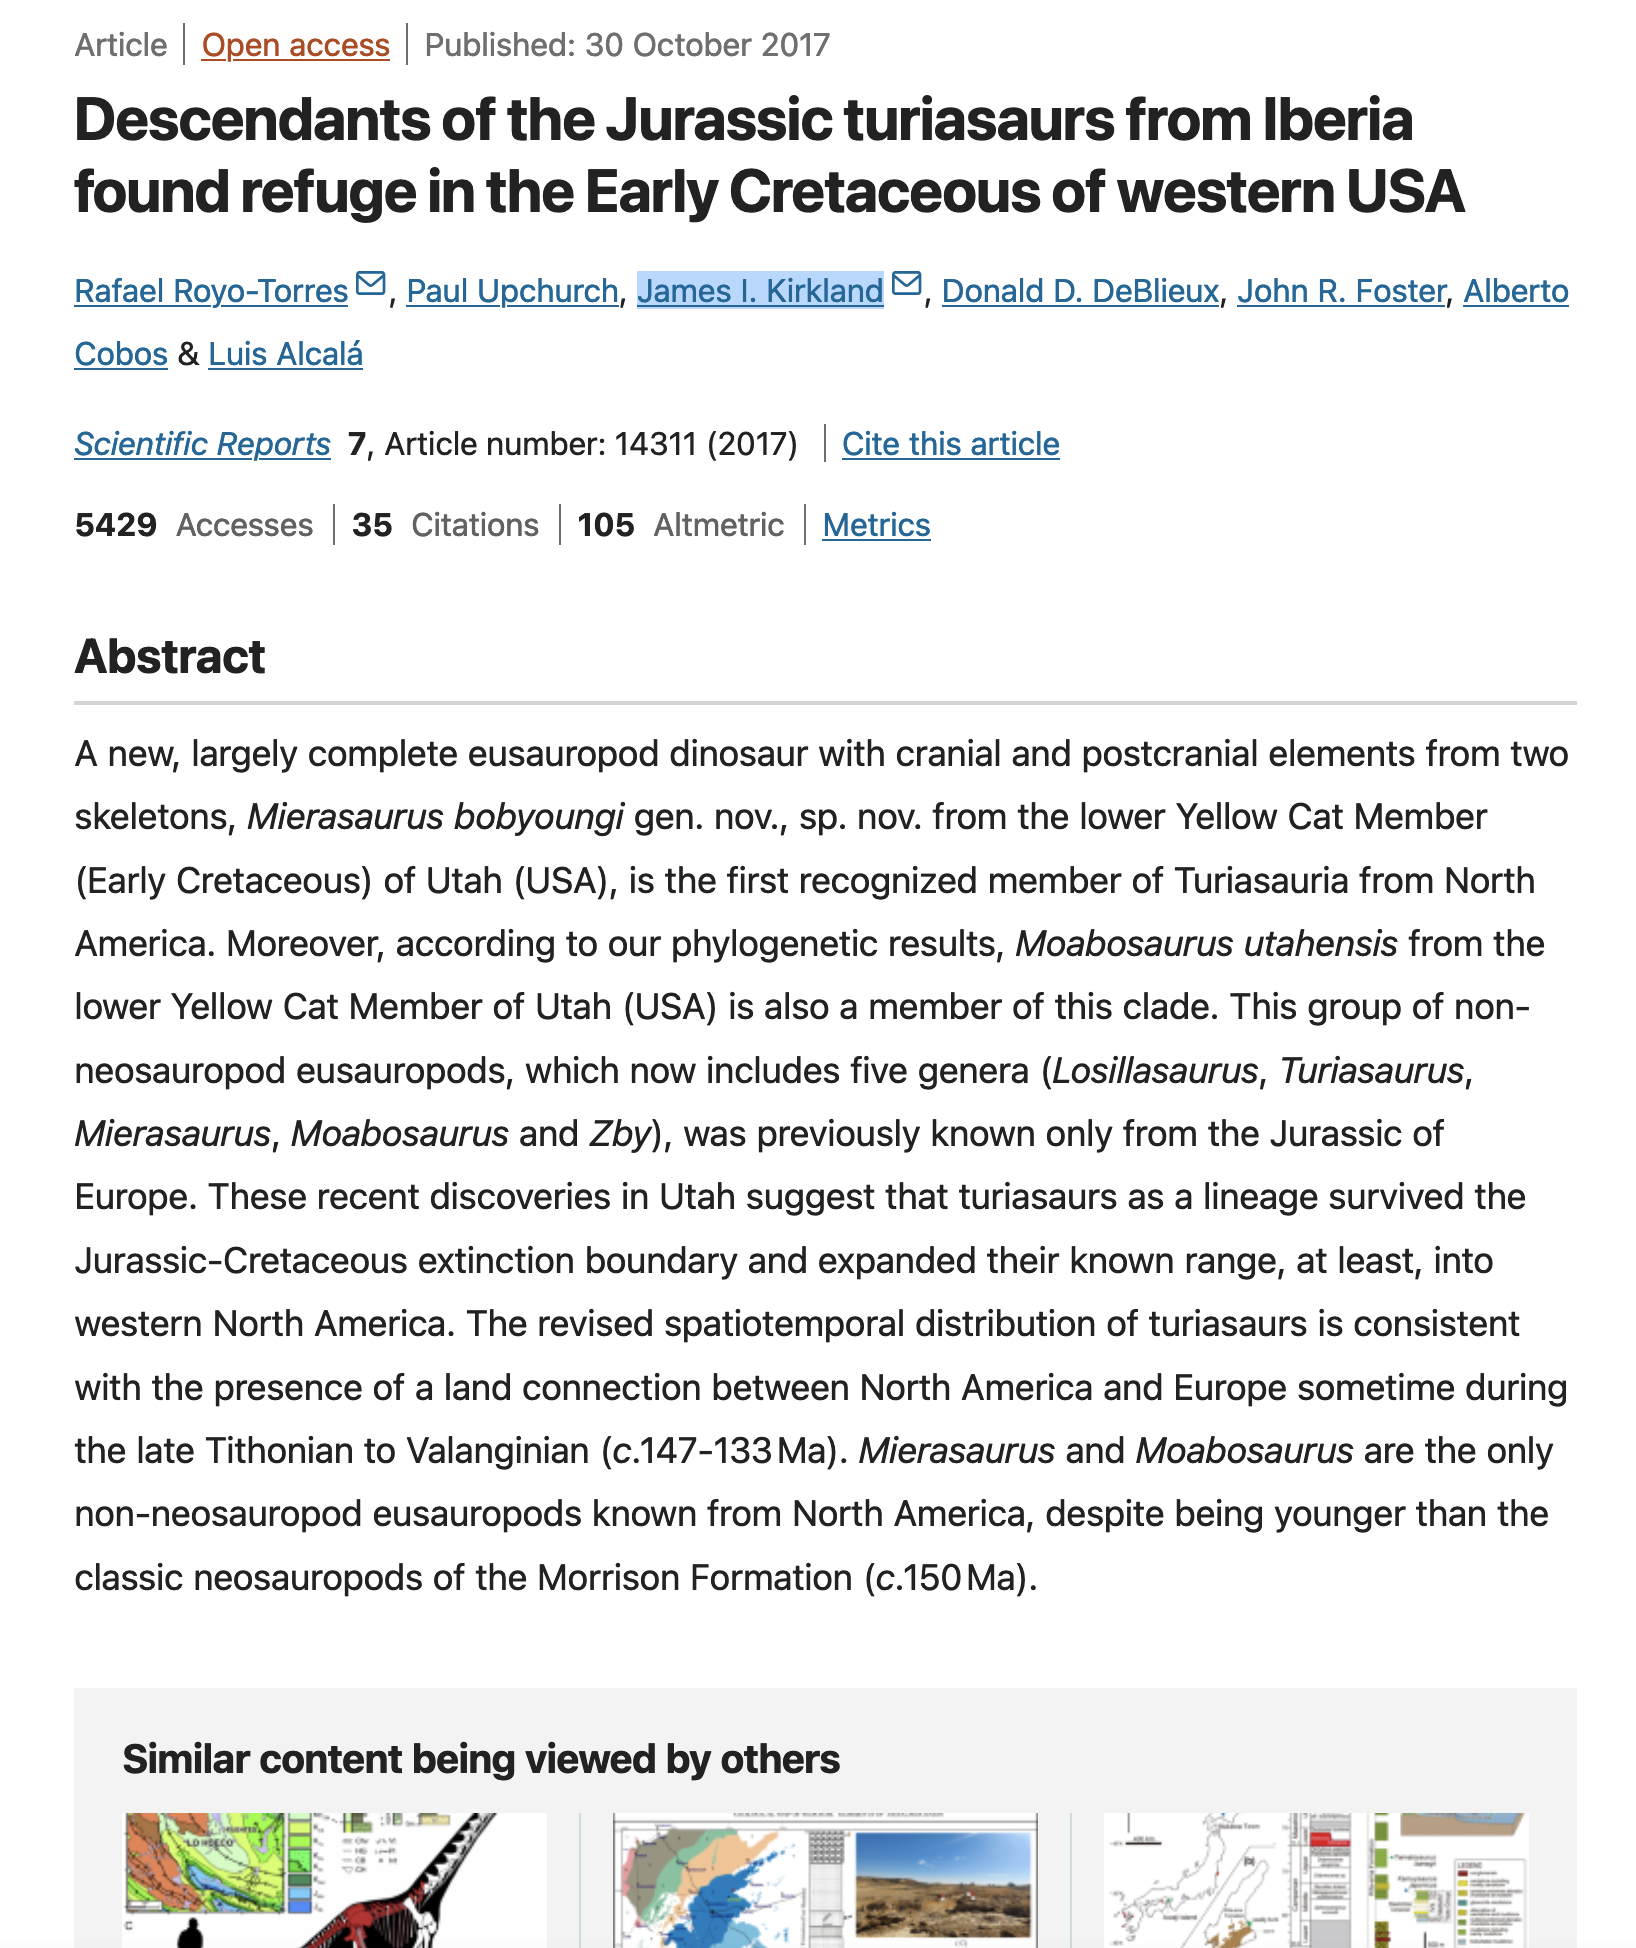
\includegraphics[width=0.8\textwidth]{figures/nature.png}
\end{figure}

\section{Utah Raptor}
\insertmydocument{subsection}{Context}{}{jim.pdf}


\chapter{My Resume}
\insertmydocument{chapter}{Numerai}{}{linkedin-resume-long.pdf}

% turtle pictures
\chapter{Charlie Summer's Art Car}

\section{Lost Art/Bogus Journey's game}
\href{https://lostartofstorytelling.com/?location=Man}{Lost Art of Storytelling}

\section{The Art Car}

\begin{figure}
    \centering
    
\includegraphics[width=0.8\textwidth]{figures/turtle_pics/pin.jpg}
\end{figure}

\begin{figure}
    \centering
    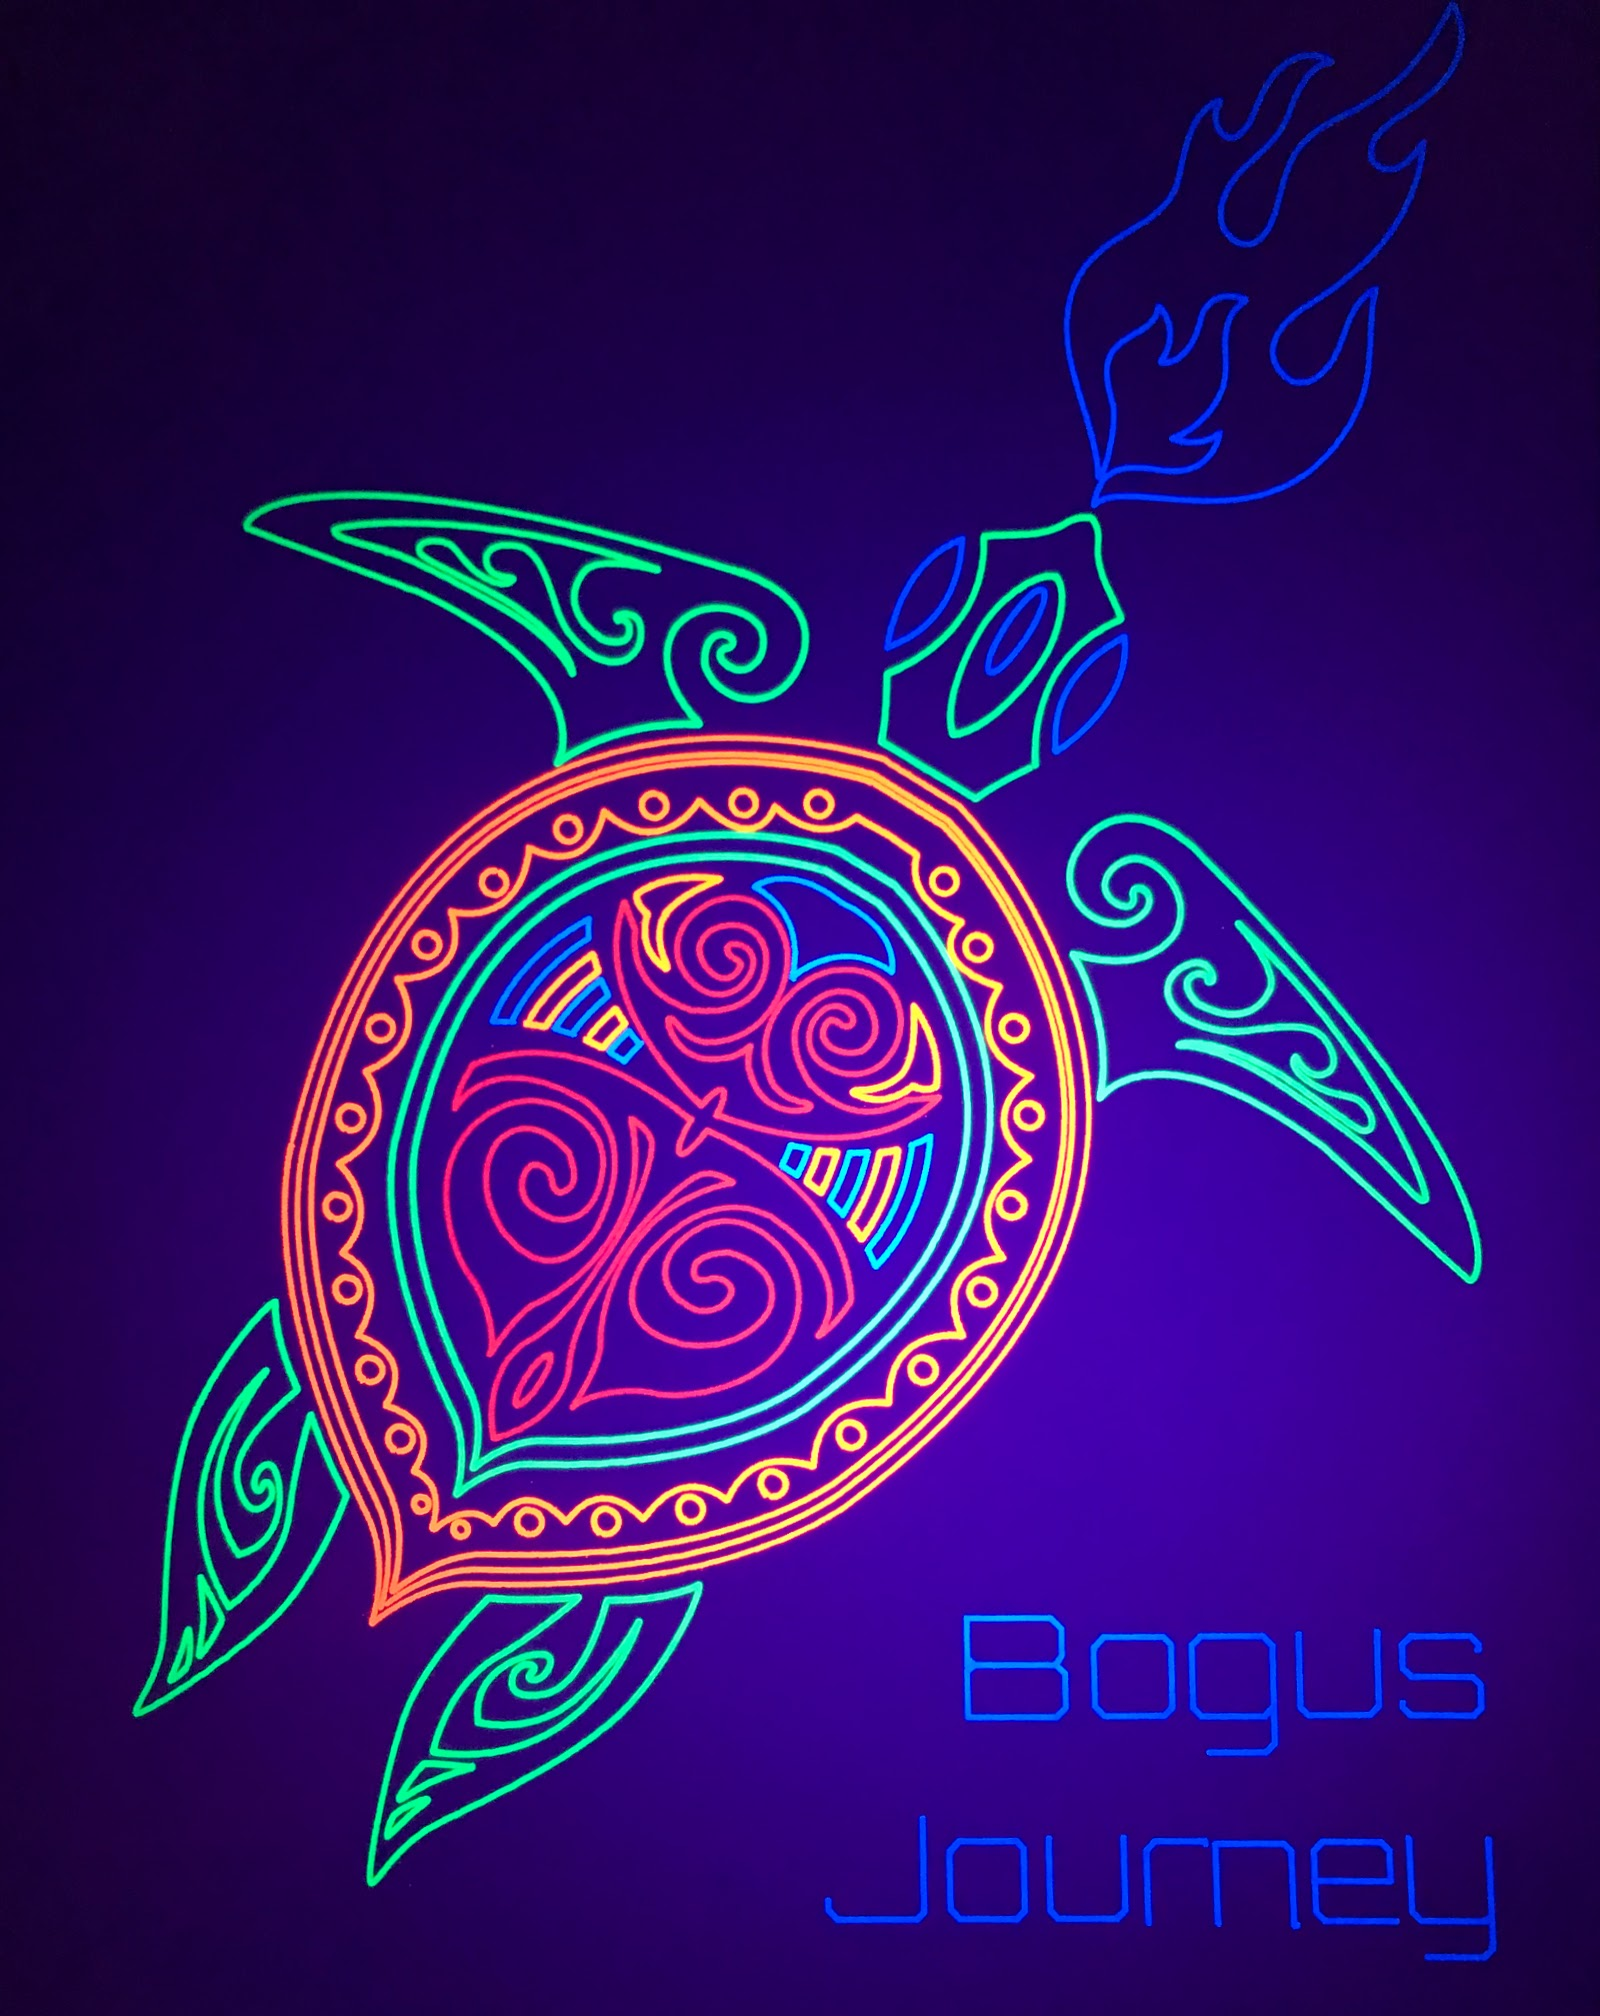
\includegraphics[width=0.8\textwidth]{figures/turtle_pics/poster1.jpg}
\end{figure}

\begin{figure}
    \centering
    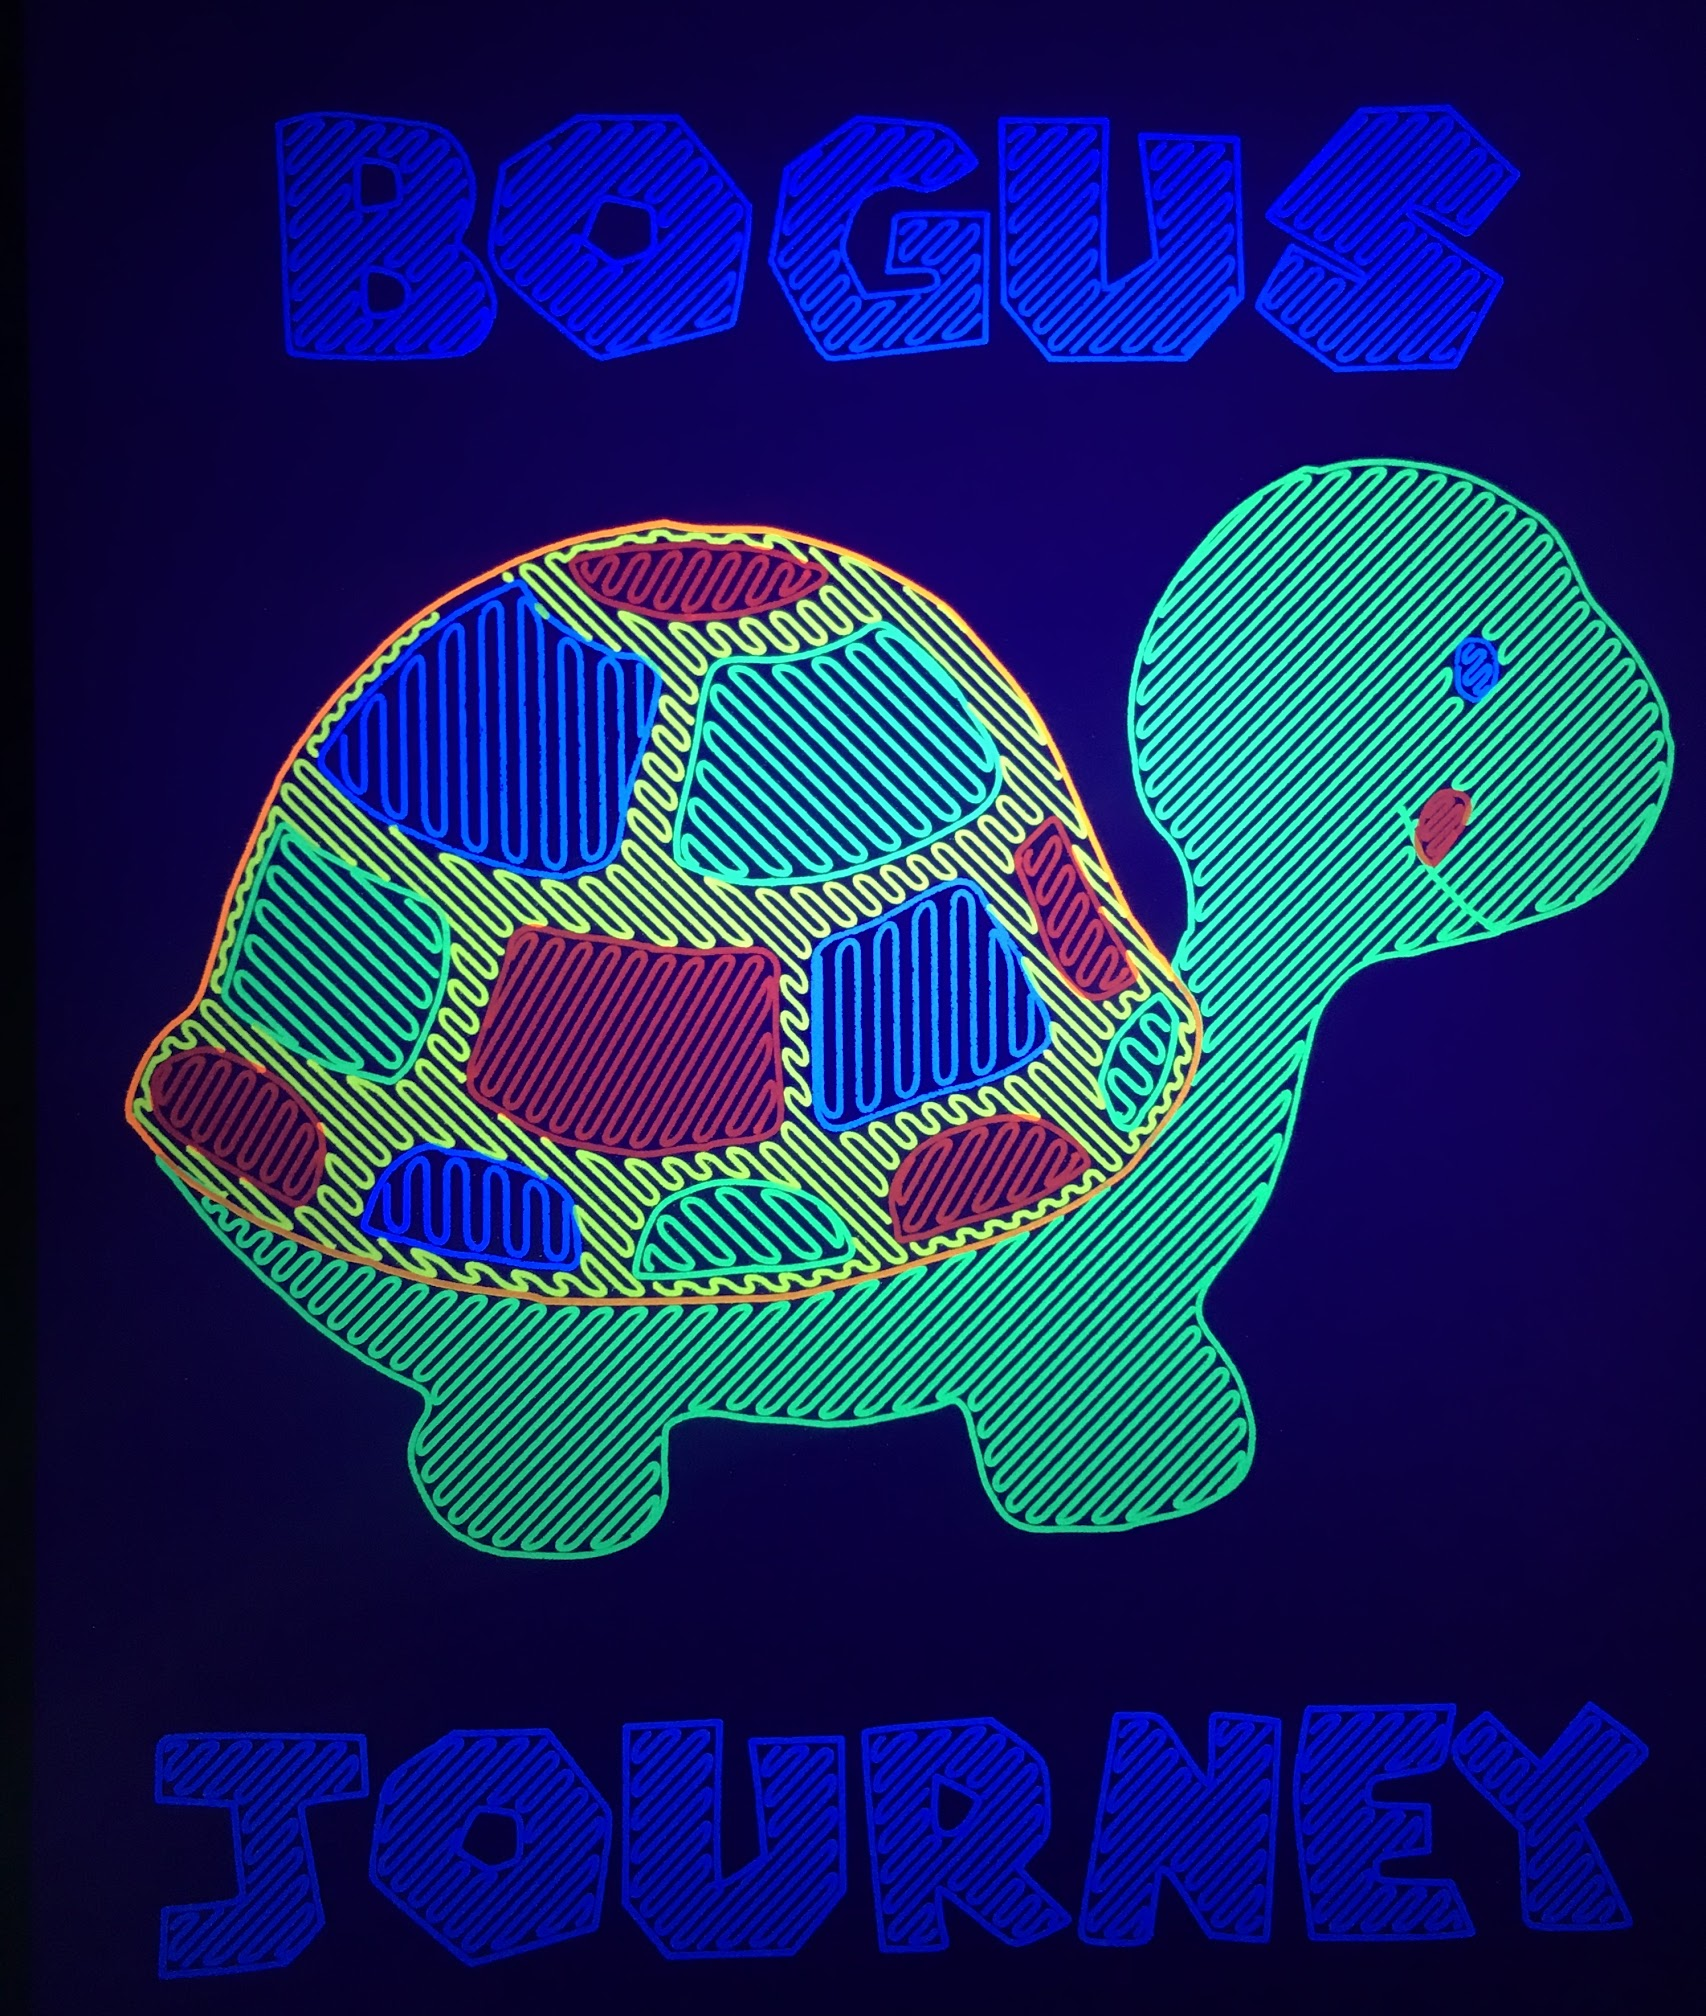
\includegraphics[width=0.8\textwidth]{figures/turtle_pics/poster2.jpg}
\end{figure}

\begin{figure}
    \centering
    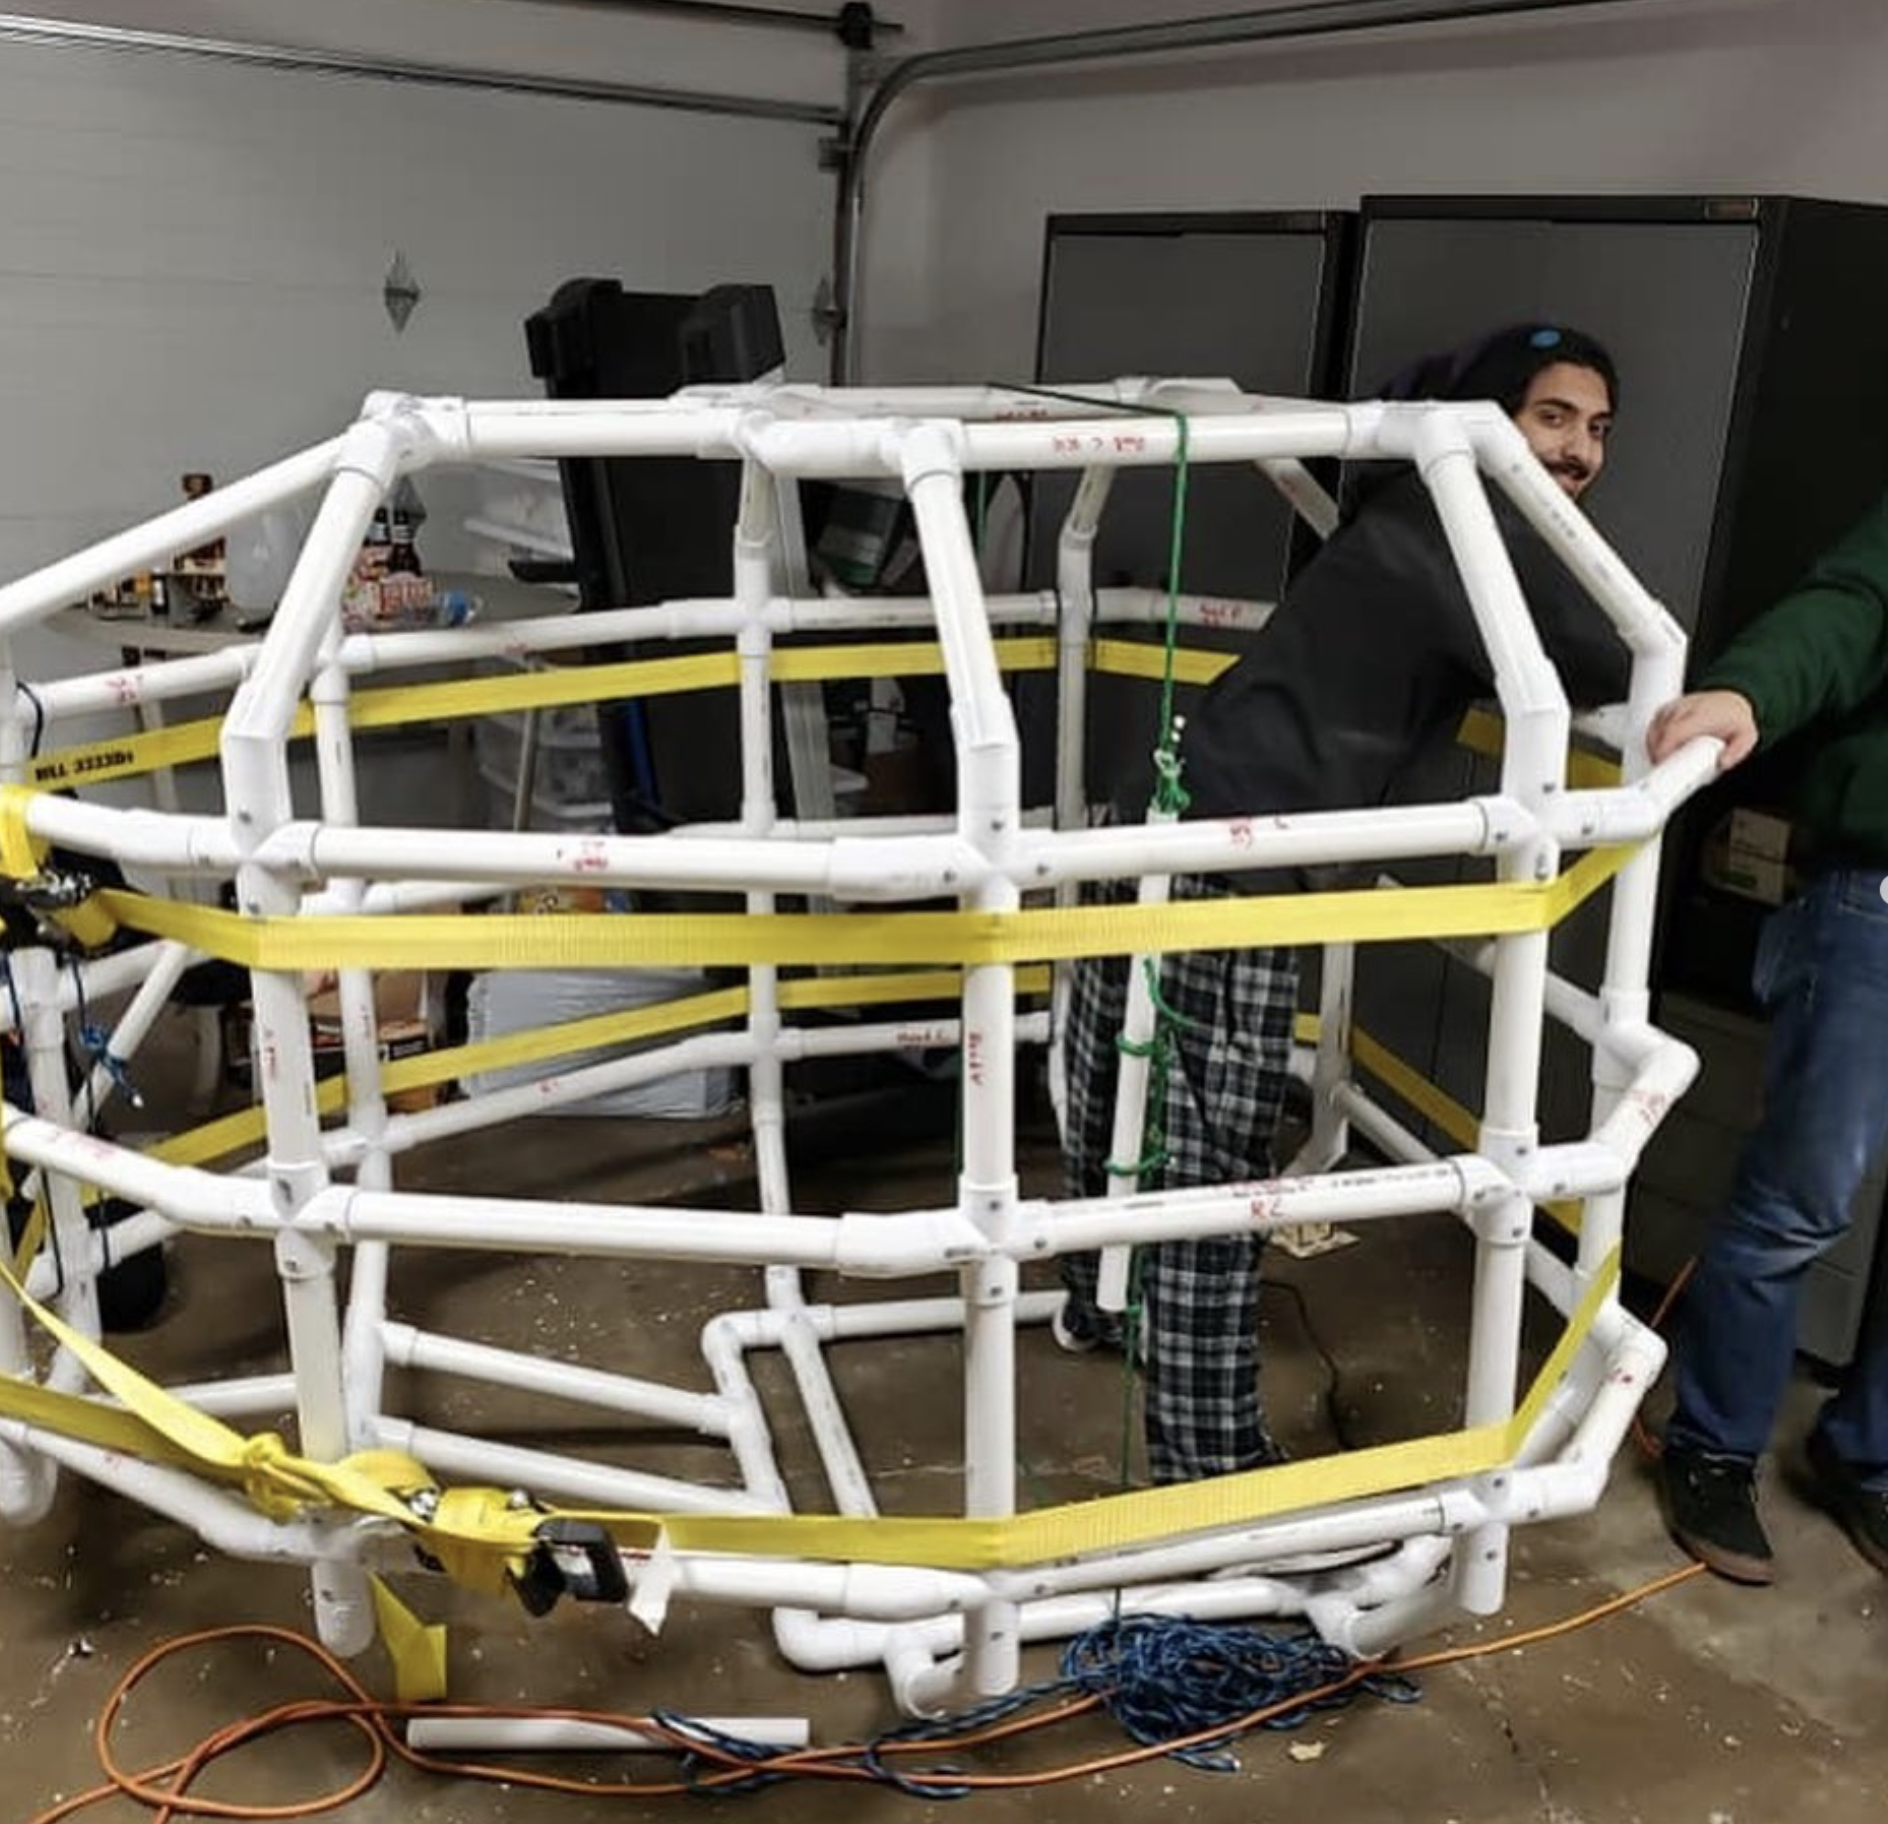
\includegraphics[width=0.8\textwidth]{figures/turtle_pics/s1.png}
\end{figure}

\begin{figure}
    \centering
    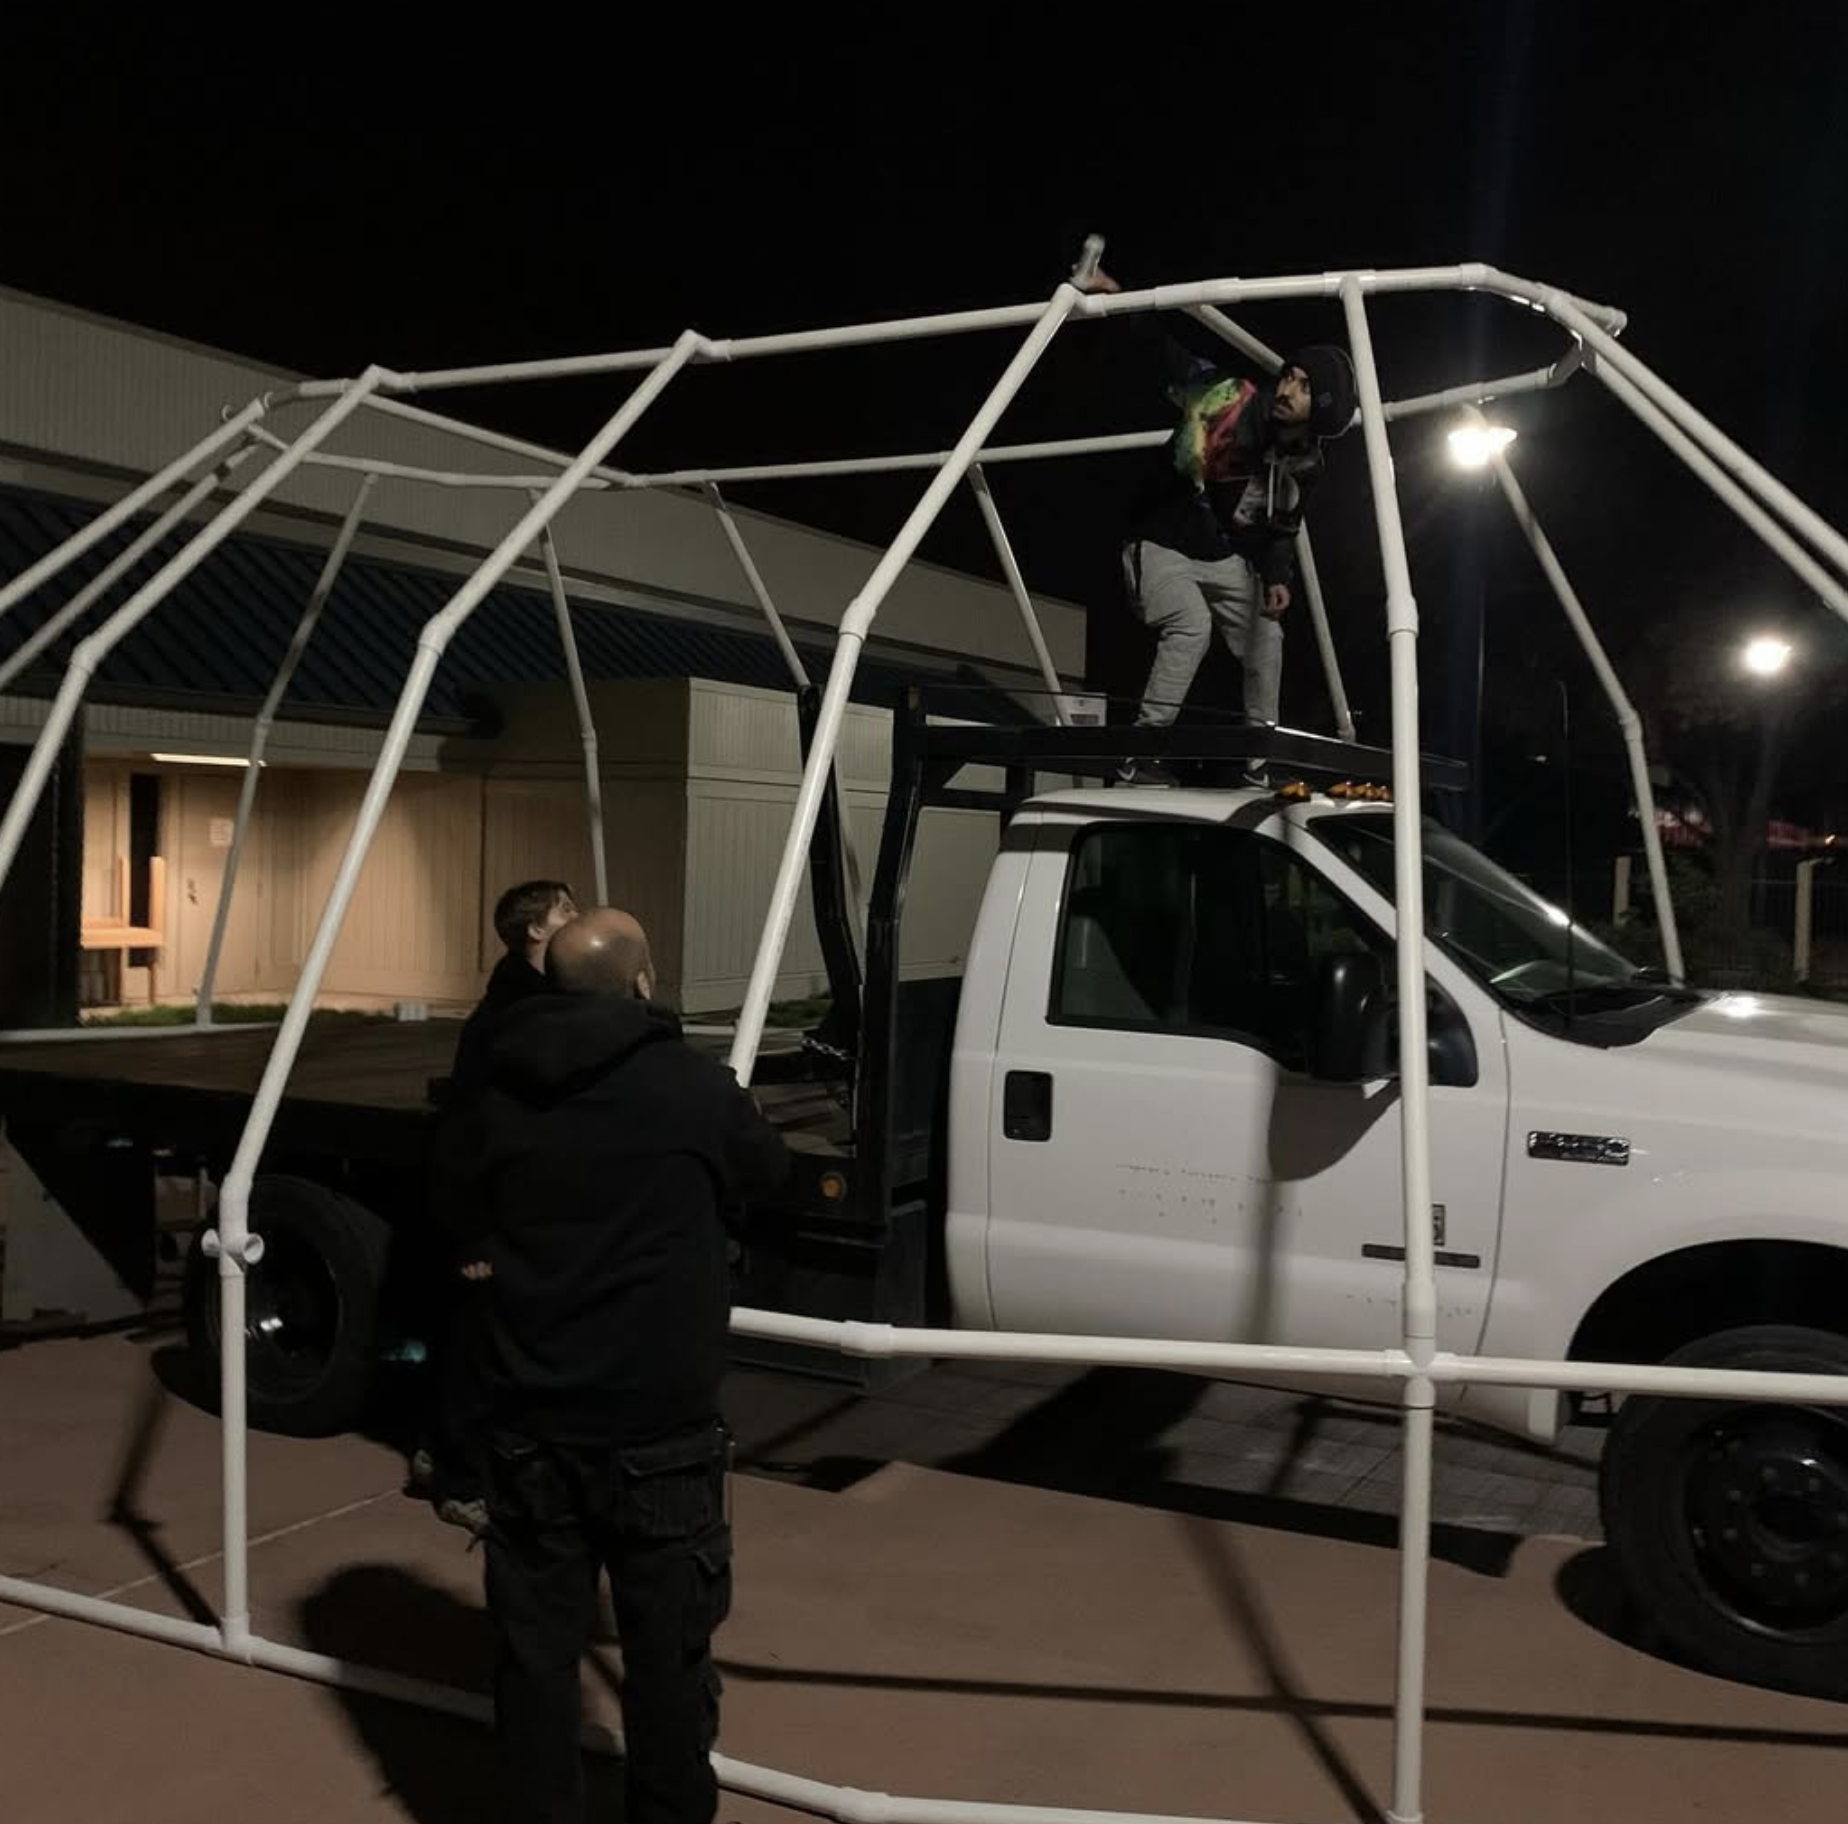
\includegraphics[width=0.8\textwidth]{figures/turtle_pics/s2.png}
\end{figure}

\begin{figure}
    \centering
    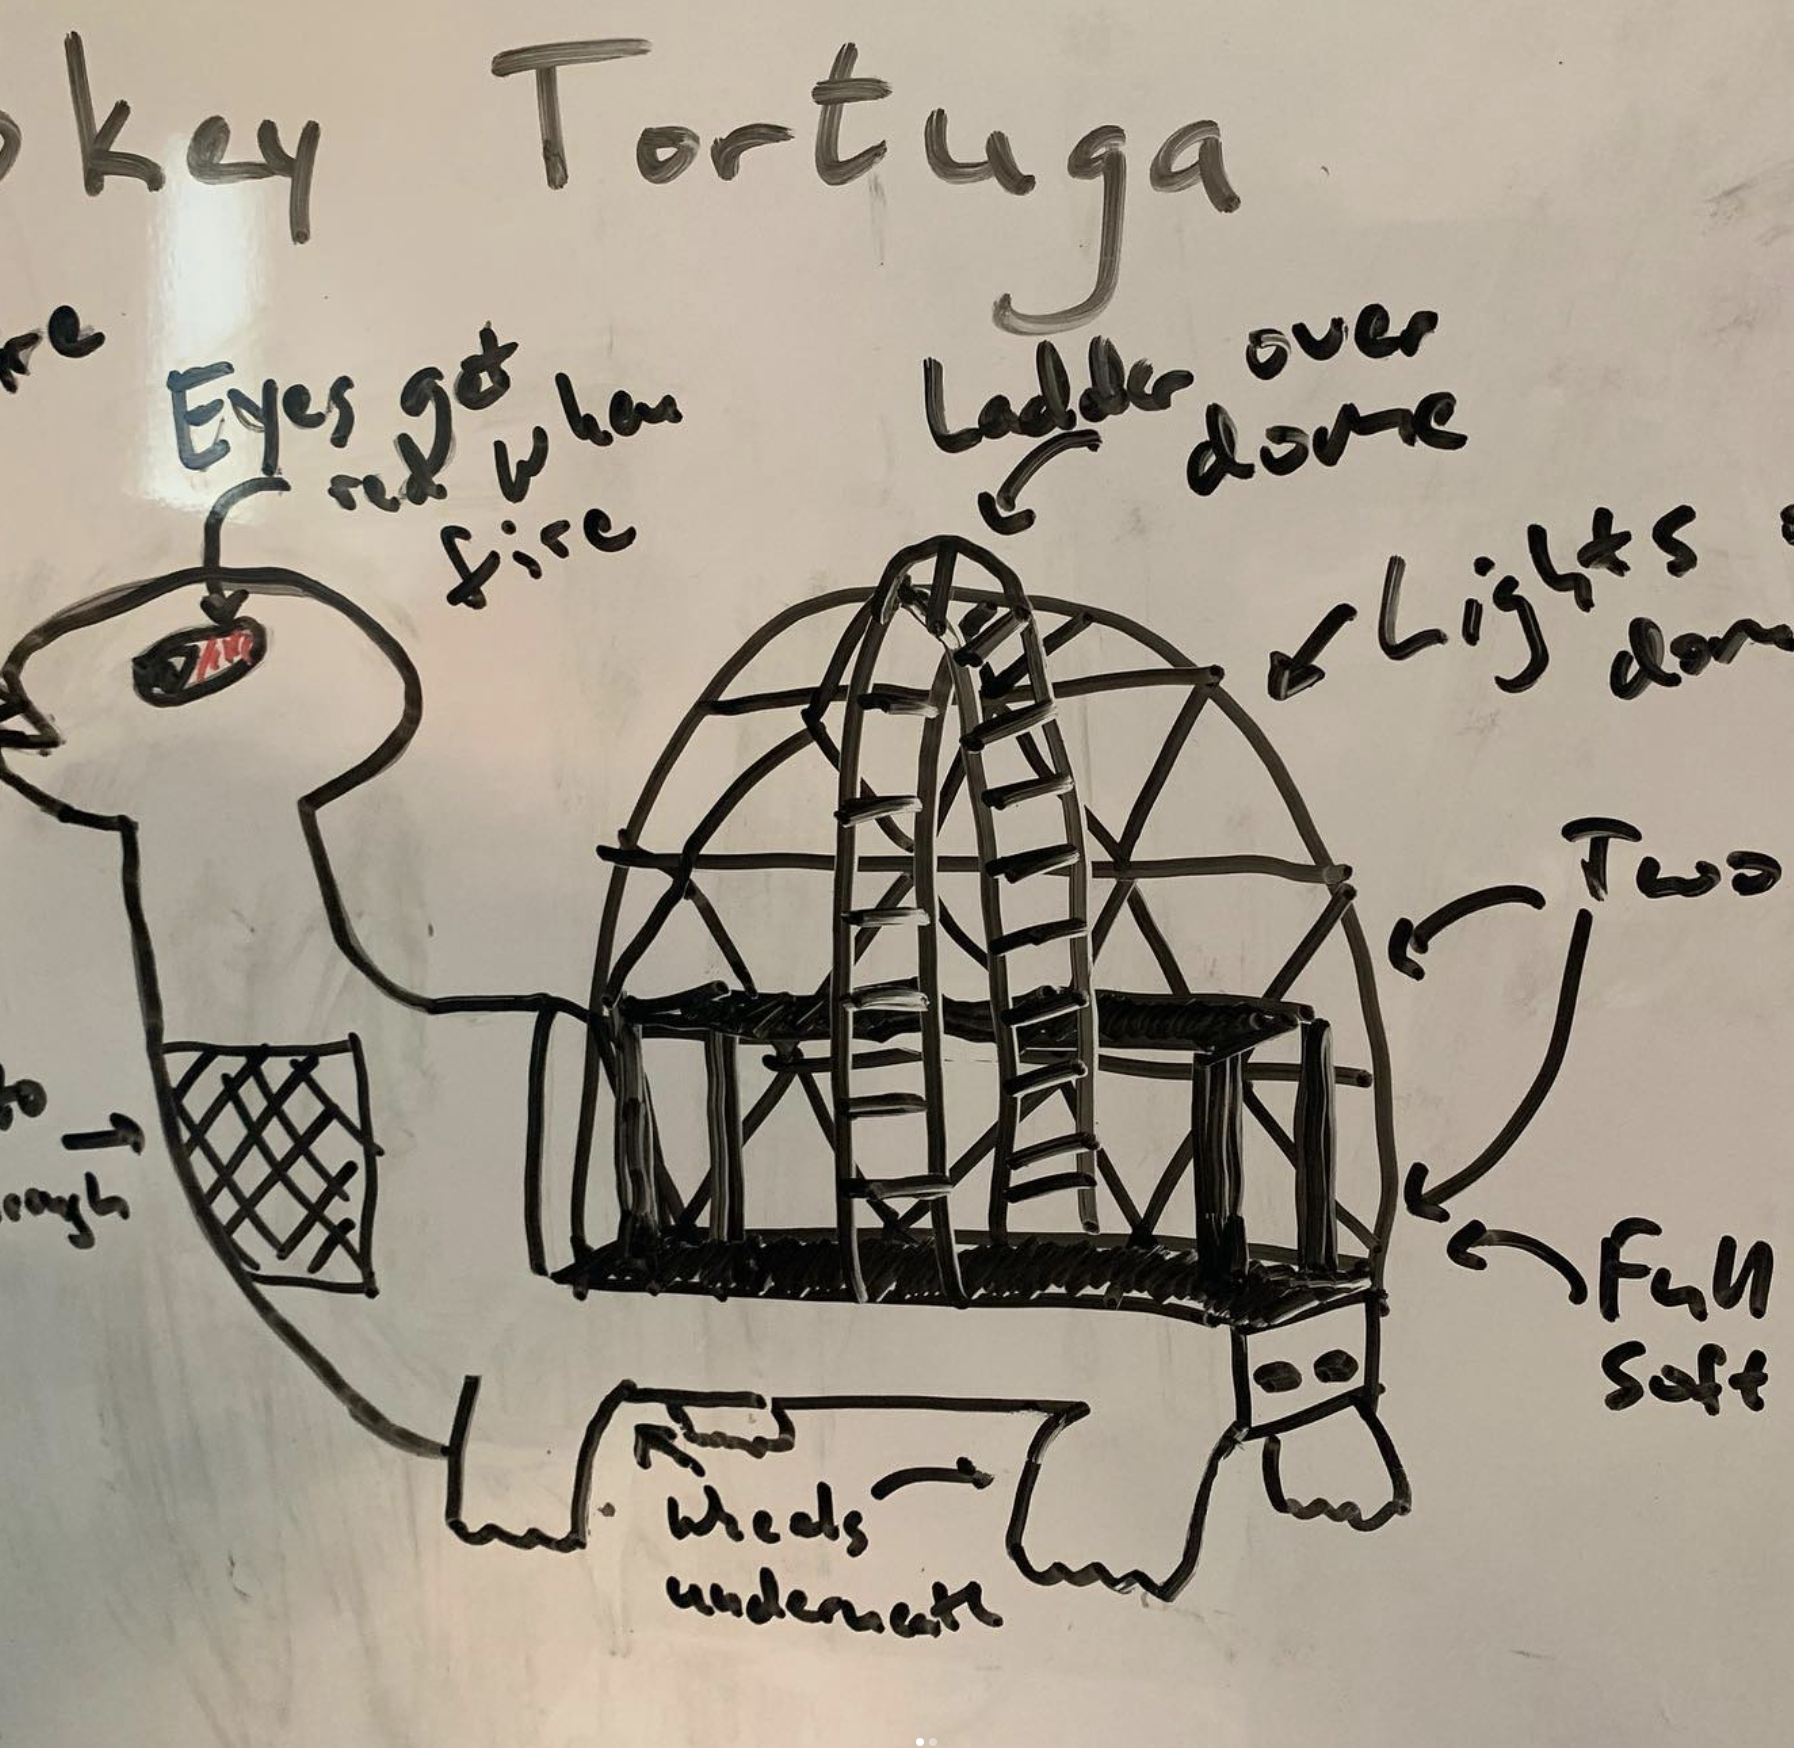
\includegraphics[width=0.8\textwidth]{figures/turtle_pics/s3.png}
\end{figure}

\begin{figure}
    \centering
    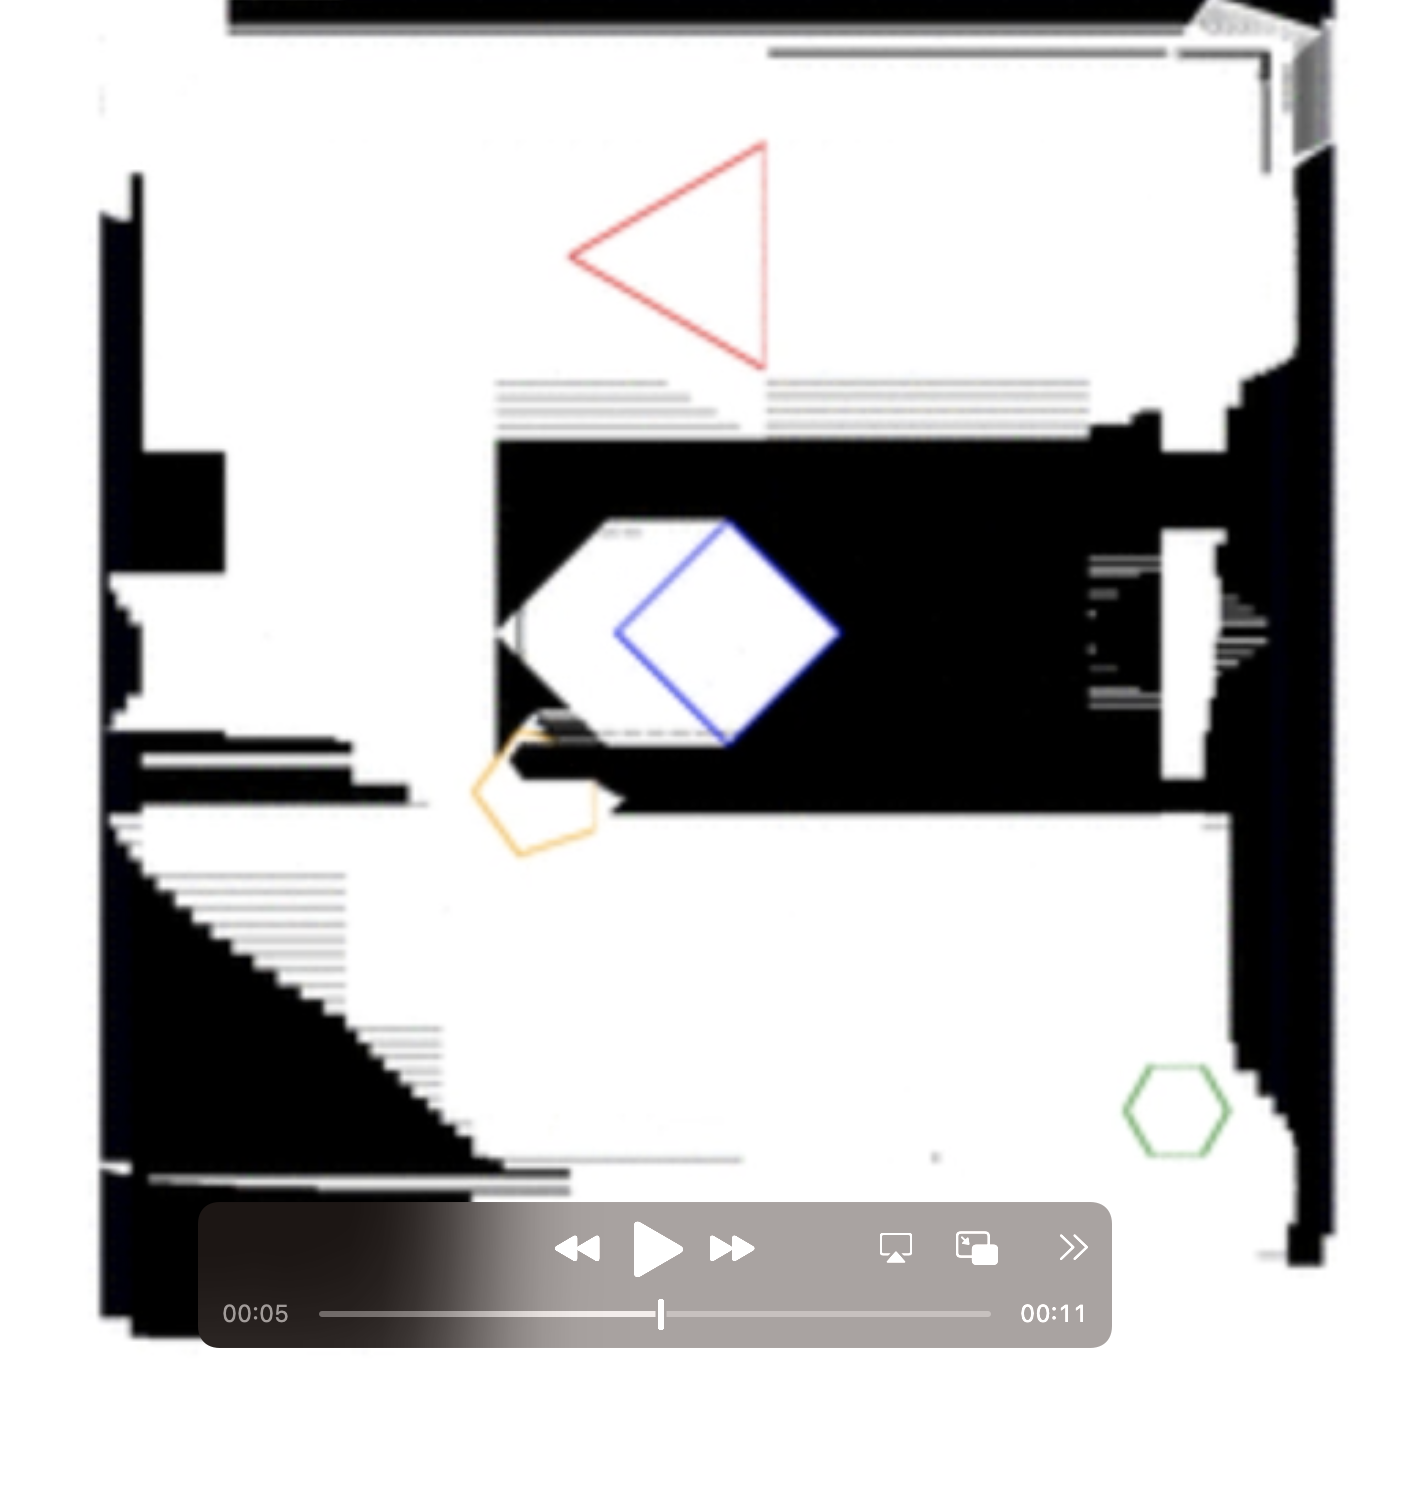
\includegraphics[width=0.8\textwidth]{figures/turtle_pics/s4.png}
\end{figure}

\begin{figure}
    \centering
    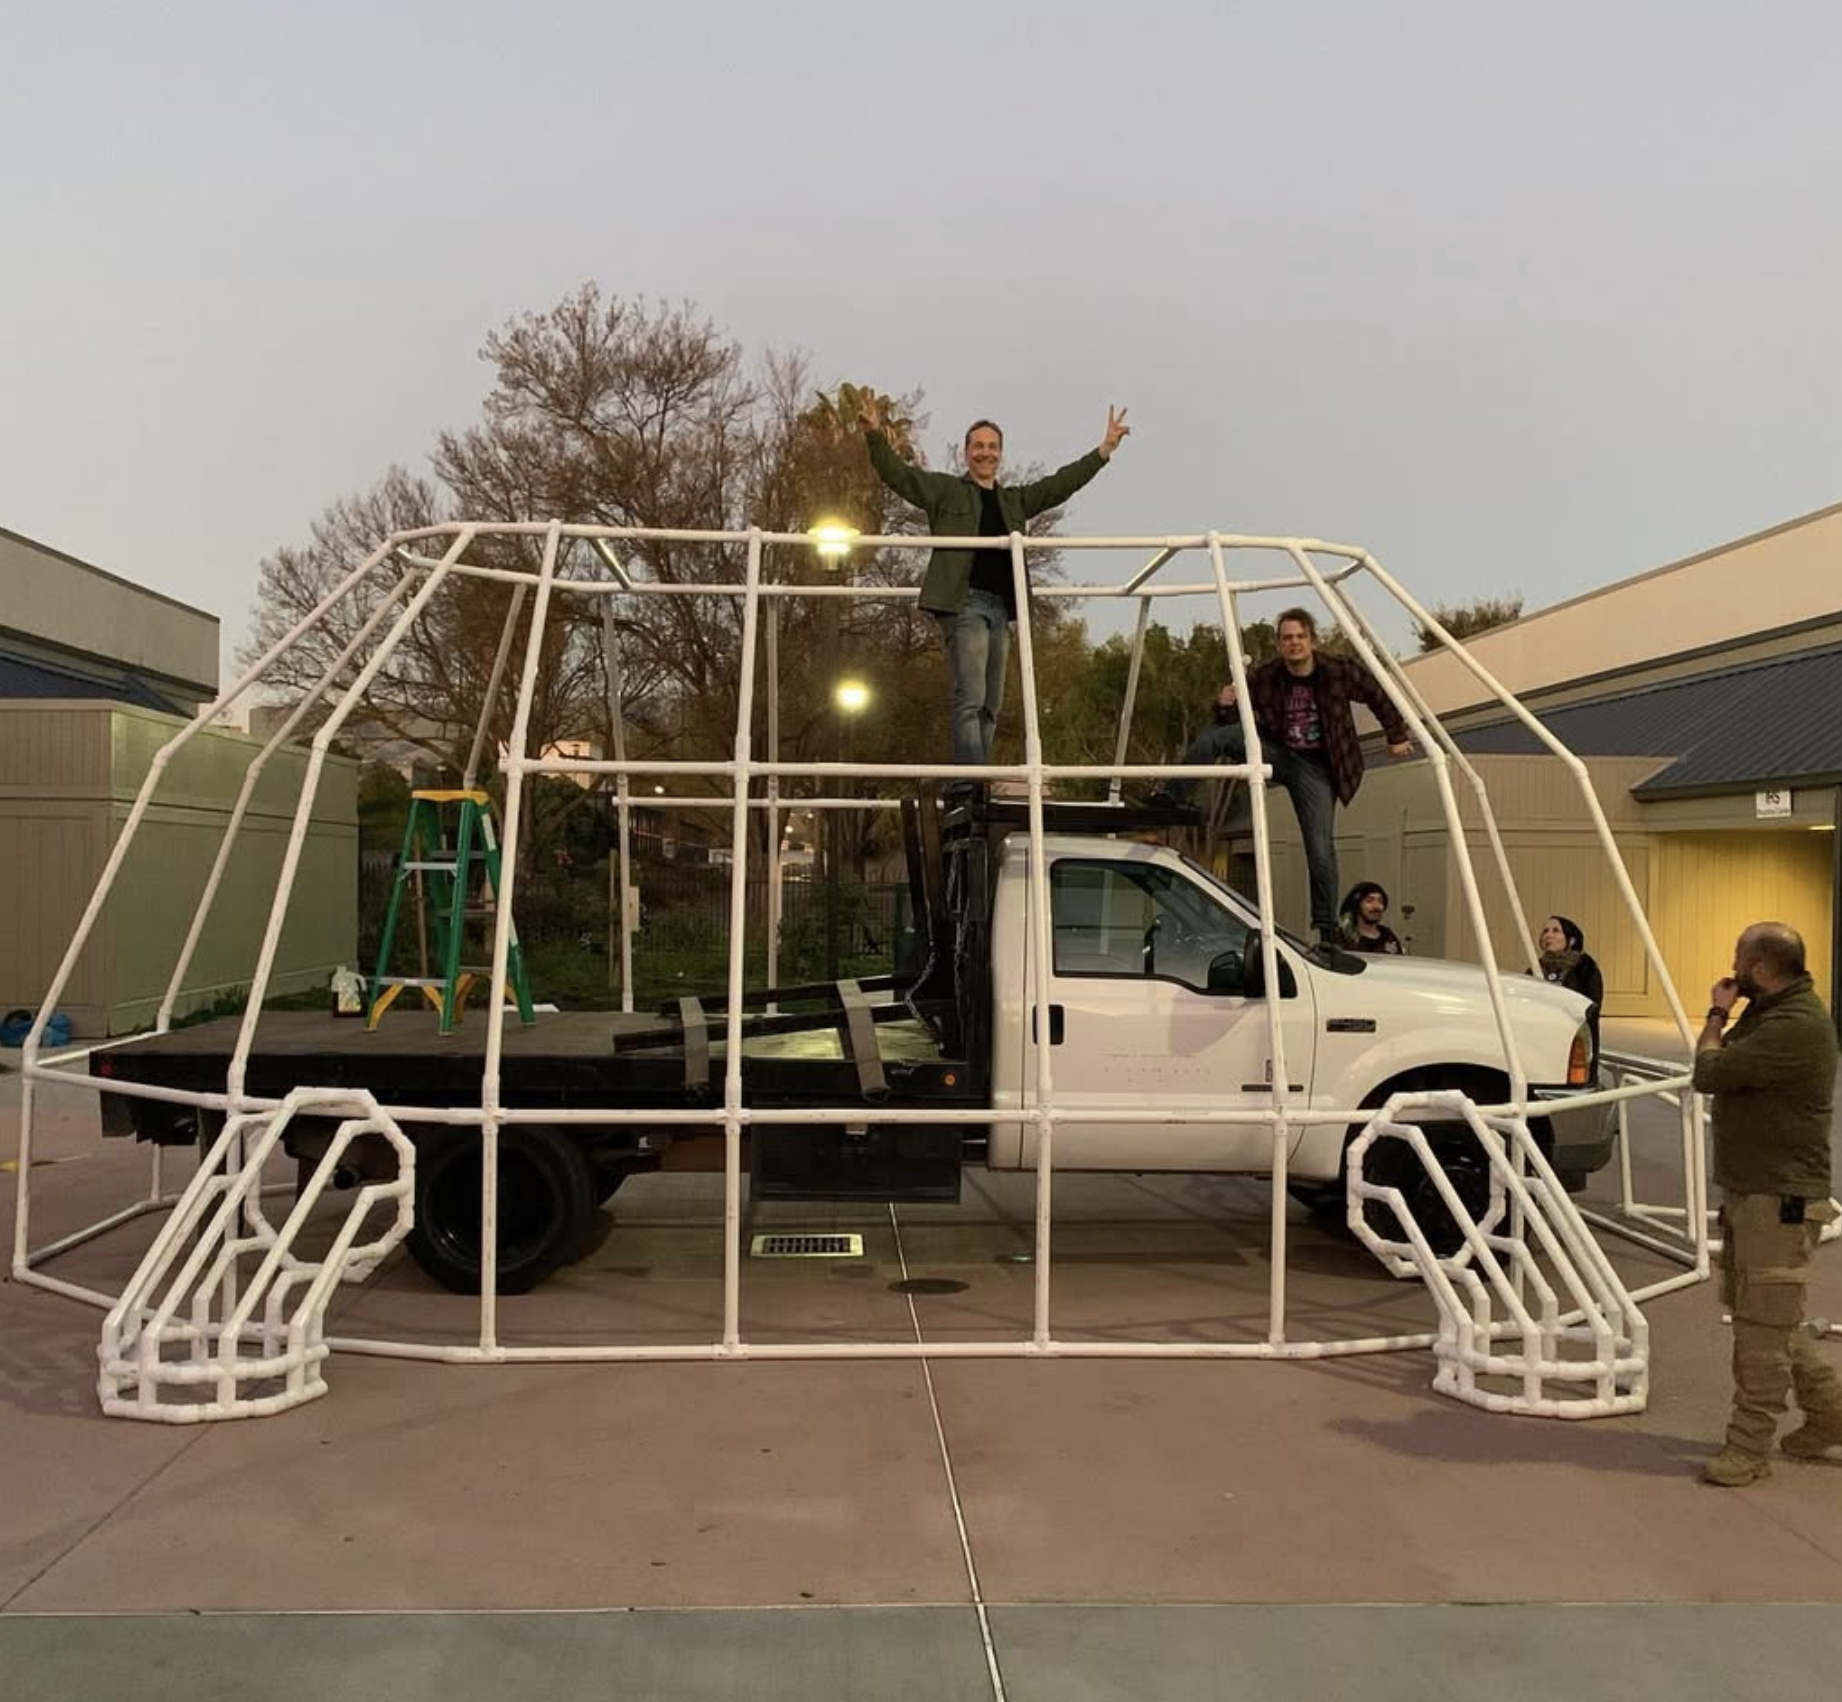
\includegraphics[width=0.8\textwidth]{figures/turtle_pics/s5.png}
\end{figure}



\chapter{Well it's Greek to me now..}
\insertmydocument{chapter}{Well it's Greek to me now..}{}{quantum.pdf}

\chapter{Phantasmagoria}
\href{https://archive.org/details/phantasmorgia/}{Phantasmagoria by Nagarjuna}



\begin{figure}
    \centering
    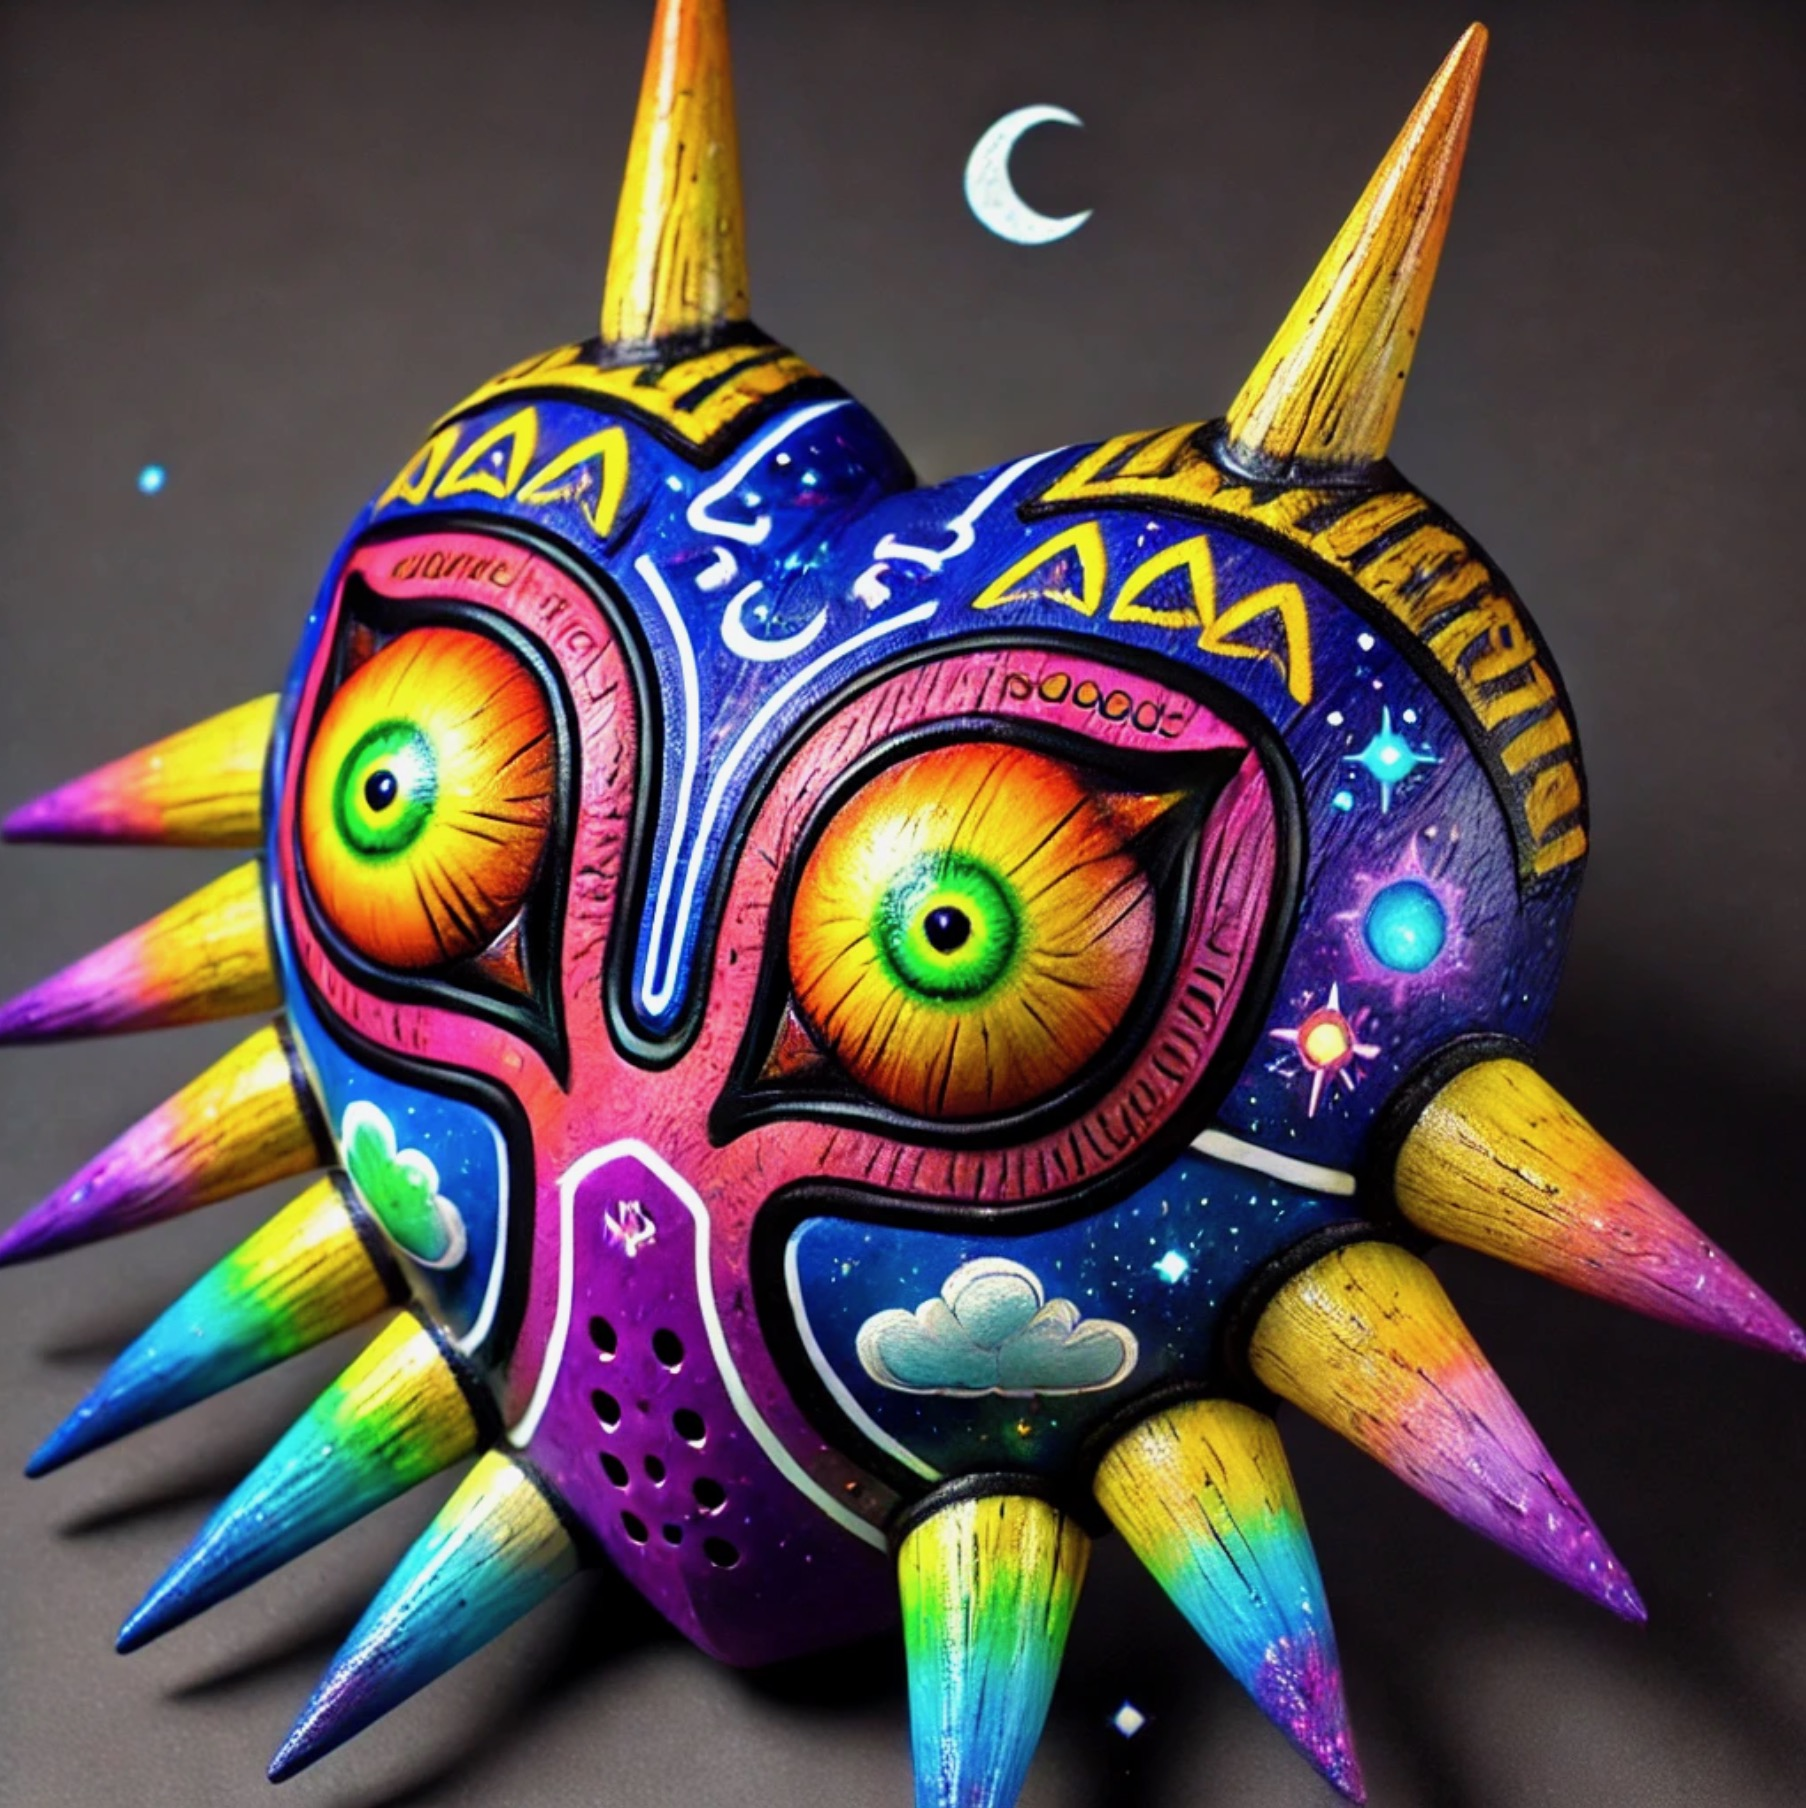
\includegraphics[width=0.8\textwidth]{figures/mask.jpeg}
    \caption{A placeholder image for \cite{oxman}}
\end{figure}

\bibliographystyle{plain} % or any other BibTeX style you prefer
\bibliography{/Users/gnb/Projects/principa-master-localcomp/references/references.bib}

\appendix

\clearpage
\chapter{Dedication outro.}
\label{outchant}
\thispagestyle{plain}

\texttt{
By means of our meritorious deeds,\\
\\
May the Suffering be free from Suffering\\
May the Fear-Struck be free from Fear\\
May the Grieving be free from Grief\\
So too may all Being-Be.\\
From the highest realms of existence to the lowest,\\
May all being arisen in these realms,\\
With form and without form,\\
With perception and without perception,\\
Be released from all Suffering,\\
And attain to Perfect Peace\\
May all being be free from suffering\\
\\
Sadu! Sadu! Sadu!
}

\begin{figure}
    \centering
    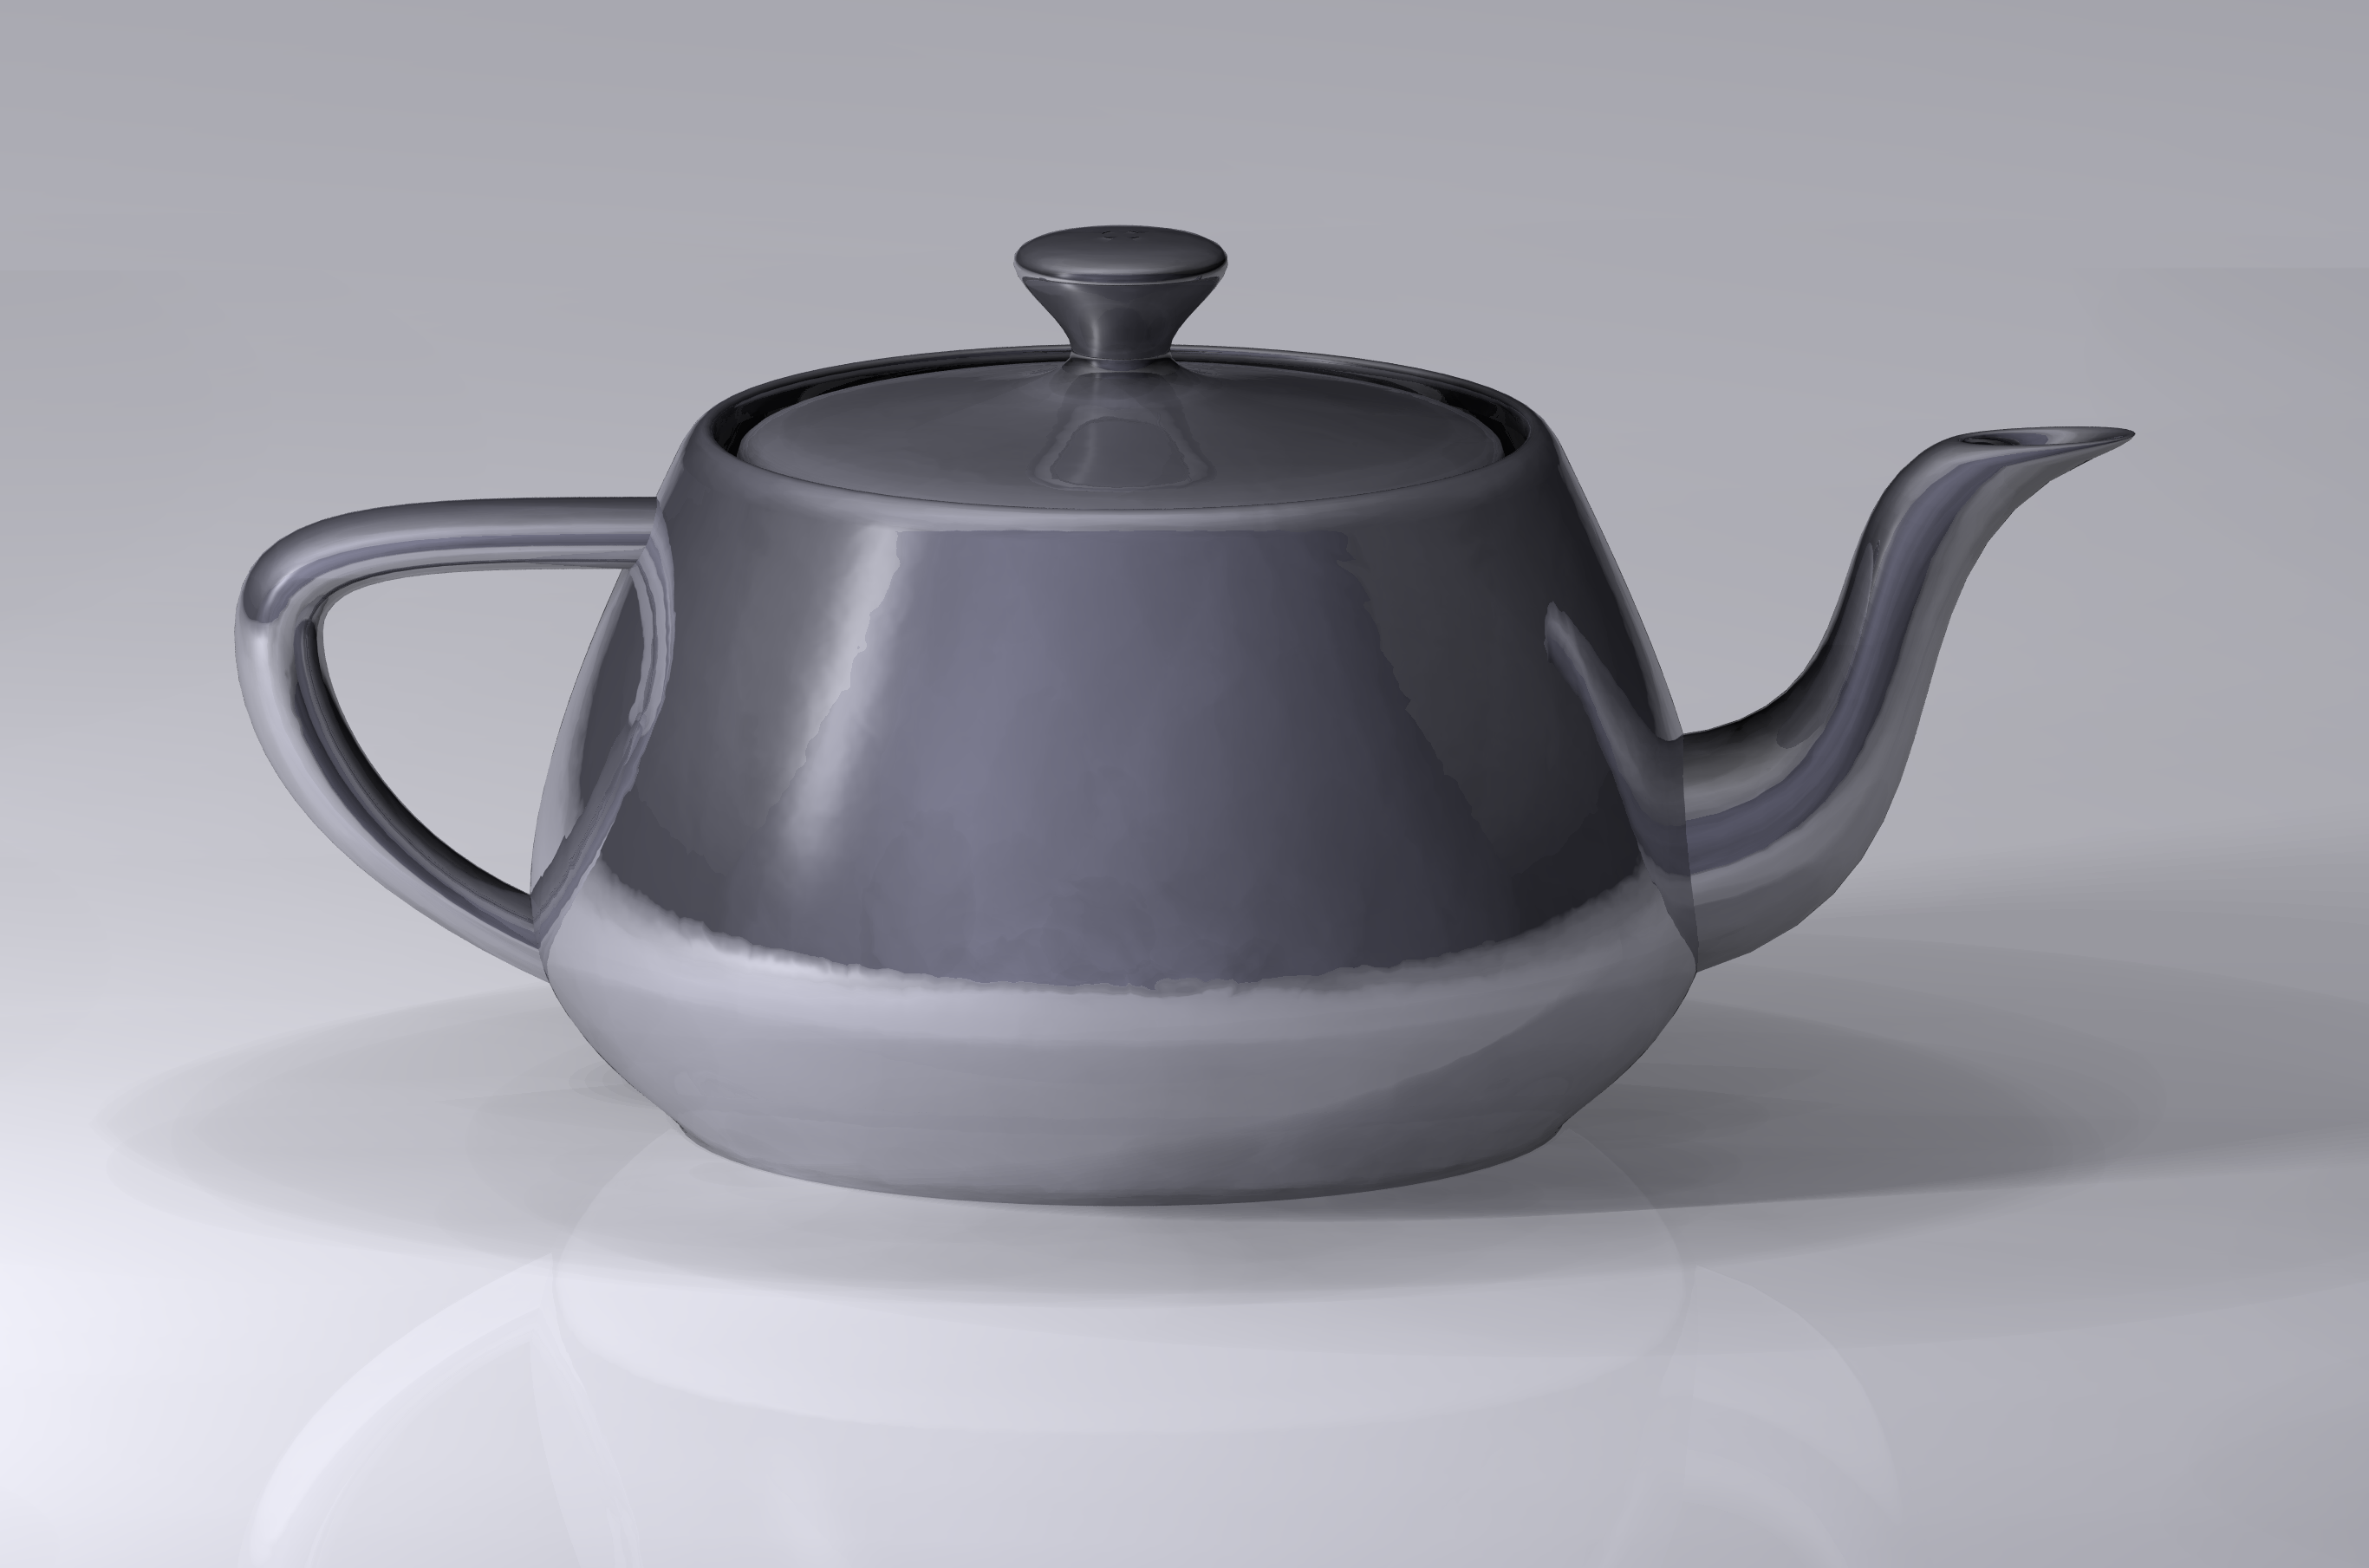
\includegraphics[width=0.8\textwidth]{figures/utah.png}
    \caption{A Utah Teapot \cite{teapot}}
\end{figure}

\begin{figure}
    \centering
    
\includegraphics[width=0.8\textwidth]{figures/aocp.jpg}
    \caption{It can't be that hard, can it? Did you try reading the manuel? \cite{eulerarchive}}
\end{figure}

\begin{figure}
    \centering
    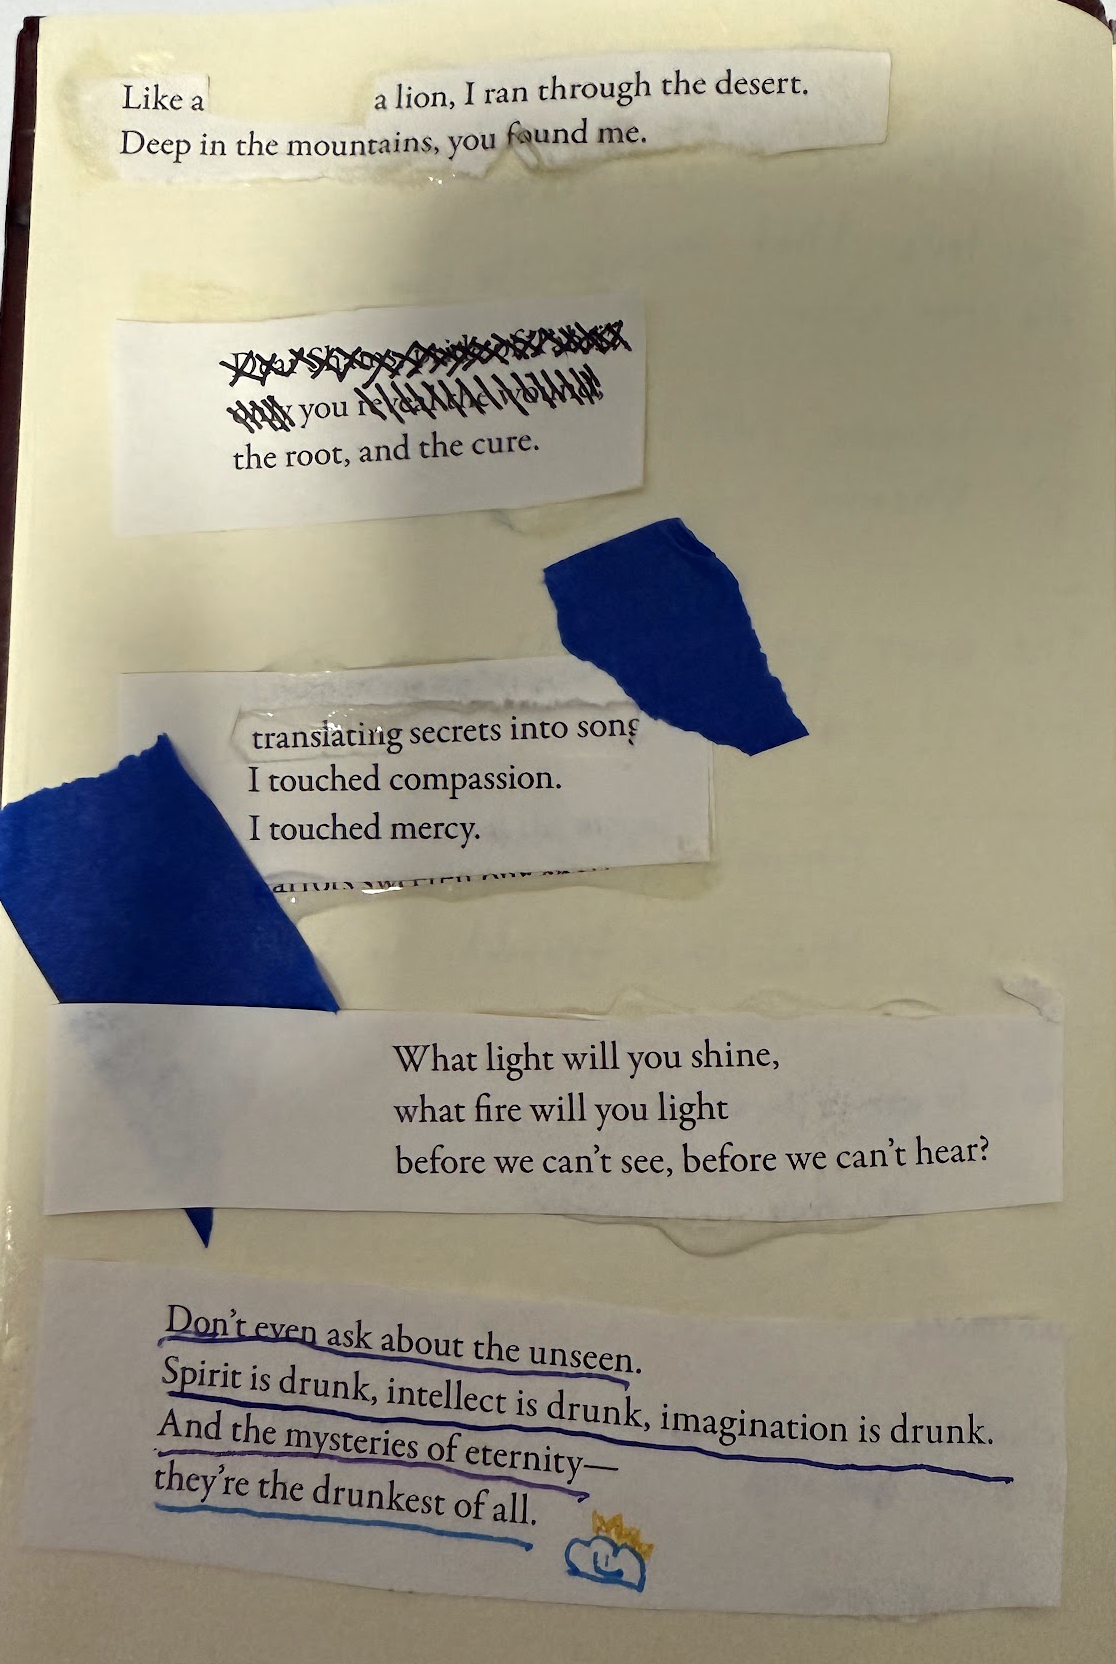
\includegraphics[width=0.8\textwidth]{figures/rumi_gold.png}
    \caption{\cite{gafori}}
\end{figure}

\end{document}
